\documentclass[a4paper]{article}
\usepackage[utf8]{inputenc}
\usepackage[margin=1in]{geometry}
\usepackage{setspace}
\usepackage{amsmath}
\usepackage{amssymb}
\usepackage{graphicx}
\usepackage{tikz}
\usepackage{array}



\title{Chapter 11\\Complex Variable Theory}
\author{solutions by Hikari}
\date{September 2021}

\begin{document}

\newcommand{\pdv}[2]{\frac{\partial#1}{\partial#2}}
\newcommand{\V}{\mathbf}
\newcommand{\del}{\boldsymbol{\nabla}}

%dashint
\def\Xint#1{\mathchoice
   {\XXint\displaystyle\textstyle{#1}}%
   {\XXint\textstyle\scriptstyle{#1}}%
   {\XXint\scriptstyle\scriptscriptstyle{#1}}%
   {\XXint\scriptscriptstyle\scriptscriptstyle{#1}}%
   \!\int}
\def\XXint#1#2#3{{\setbox0=\hbox{$#1{#2#3}{\int}$}
     \vcenter{\hbox{$#2#3$}}\kern-.5\wd0}}
\def\ddashint{\Xint{\;\,-}}
\def\dashint{\Xint-}


\maketitle

\section*{11.2 Cauchy-Riemann Conditions}

\paragraph{11.2.1}
\[
\pdv{u}{x}=1\neq\pdv{v}{y}=0
\]
so it is not analytic.

\paragraph{11.2.2}
The real and imaginary parts of analytic functions satisfy Laplace's equation, and it has been shown in Section 9.5 that functions satisfying Laplace's equation cannot have a maximum or minimum within the bounded region.

\paragraph{11.2.3}
(a)
\begin{align*}
    \pdv{u}{x} & =\pdv{v}{y}=3x^2-3y^2\\
    -\pdv{u}{y} & =\pdv{v}{x}=6xy
\end{align*}
\[
v(x,y)=3x^2y-y^3
\]
\[
w(z)=x^3-3xy^2+i(3x^2y-y^3)=(x+iy)^3=z^3
\]

(b)
\begin{align*}
    & \pdv{u}{x}=\pdv{v}{y}=-e^{-y}\sin x\\
    & \pdv{u}{y}=-\pdv{v}{x}=-e^{-y}\cos x
\end{align*}
\[
u(x,y)=e^{-y}\cos x
\]
\[
w(z)=e^{-y}\cos x+ie^{-y}\sin x=e^{i(x+iy)}=e^{iz}
\]

\paragraph{11.2.4}
$w_1$ analytic:
\[
\pdv{u}{x}=\pdv{v}{y}\qquad \pdv{u}{y}=-\pdv{v}{x}
\]
$w_1^*$ analytic:
\[
\pdv{u}{x}=-\pdv{v}{y}\qquad \pdv{u}{y}=\pdv{v}{x}
\]
so 
\[
\pdv{u}{x}=\pdv{u}{y}=\pdv{v}{x}=\pdv{v}{y}=0
\]
which means $u(x,y)$ and $v(x,y)$ are constants.

\paragraph{11.2.5}
\[
f(z)=\frac{1}{x+iy}=\frac{x}{x^2+y^2}-i\frac{y}{x^2+y^2}
\]
\begin{align*}
    & \pdv{u}{x}=\frac{-x^2+y^2}{(x^2+y^2)^2}=\pdv{v}{y}\\
    & \pdv{u}{y}=\frac{-2xy}{(x^2+y^2)^2}=-\pdv{v}{x}
\end{align*}
so $f(z)$ is analytic (except $z=0$).

\paragraph{11.2.6}
\[
f'(z)=\frac{(\pdv{u}{x}+i\pdv{v}{x})adx+(\pdv{u}{y}+i\pdv{v}{y})bdy}{a\,dx+ib\,dy}
\]
\[
=\frac{(\pdv{u}{x}+i\pdv{v}{x})adx+(-\pdv{v}{x}+i\pdv{u}{x})bdy}{a\,dx+ib\,dy}
\]
\[
=\frac{(\pdv{u}{x}+i\pdv{v}{x})adx+(\pdv{u}{x}+i\pdv{v}{x})ibdy}{a\,dx+ib\,dy}
\]
\[
=\pdv{u}{x}+i\pdv{v}{x}
\]

\paragraph{11.2.7}
\begin{align*}
    & \delta z=e^{i\theta}\delta r+ire^{i\theta}\delta\theta\\
    & \delta f=e^{i\Theta}\delta R+iRe^{i\Theta}d\Theta
\end{align*}
\begin{align*}
    & \lim_{\delta z\to0}\frac{\delta f}{\delta z}=\lim_{\delta r\to0}\left(\frac{e^{i\Theta}\delta R}{e^{i\theta}\delta r}+\frac{iRe^{i\Theta}\delta\Theta}{e^{i\theta}\delta r} \right)=e^{i(\Theta-\theta)}\pdv{R}{r}+iRe^{i(\Theta-\theta)}\pdv{\Theta}{r}\\[3pt] 
    & \lim_{\delta z\to0}\pdv{f}{z}=\lim_{\delta\theta\to0}\left(\frac{e^{i\Theta}\delta R}{ire^{i\theta}\delta\theta}+\frac{iRe^{i\Theta}\delta\Theta}{ire^{i\theta}\delta\theta} \right)=-i\frac{e^{i(\Theta-\theta)}}{r}\pdv{R}{\theta}+\frac{Re^{i(\Theta-\theta)}}{r}\pdv{\Theta}{\theta}
\end{align*}
Equating the real and imaginary parts, we have 
\[
\pdv{R}{r}=\frac{R}{r}\pdv{\Theta}{\theta}
\]
\[
\frac{1}{r}\pdv{R}{\theta}=-R\pdv{\Theta}{r}
\]

\paragraph{11.2.8}
From Exercise 11.2.7, we have
\begin{align*}
    & \pdv{^2R}{r\partial\theta}=\pdv{}{\theta}\left(\frac{R}{r}\pdv{\Theta}{\theta}\right)=\frac{1}{r}\pdv{R}{\theta}\pdv{\Theta}{\theta}+\frac{R}{r}\pdv{^2\Theta}{\theta^2}=-R\pdv{\Theta}{r}\pdv{\Theta}{\theta}+\frac{R}{r}\pdv{^2\Theta}{\theta^2}\\
    & \pdv{^2R}{r\partial\theta}=\pdv{}{r}\left(-rR\pdv{\Theta}{r}\right)=-R\pdv{\Theta}{r}-r\pdv{R}{r}\pdv{\Theta}{r}-rR\pdv{^2\Theta}{r^2}=-R\pdv{\Theta}{r}-R\pdv{\Theta}{\theta}\pdv{\Theta}{r}-rR\pdv{^2\Theta}{r^2}
\end{align*}
Equate the two equations and divide by $rR$, we have
\[
\pdv{^2\Theta}{r^2}+\frac{1}{r}\pdv{\Theta}{r}+\frac{1}{r^2}\pdv{^2\Theta}{\theta^2}=0
\]

\paragraph{11.2.9}
(a)
$
f'(z)=\frac{\cos z}{z}-\frac{\sin z}{z^2}
$,\;
$f(z)$ is analytic at every finite $z$.
\medskip

(b)
$
f'(z)=\frac{-2z}{(z^2+1)^2}
$,\;
$f(z)$ is analytic at every finite $z$ except $z=\pm i$.
\medskip

(c)
$
f'(z)=\frac{-(2z+1)}{z^2(z+1)^2}
$,\;
$f(z)$ is analytic at every finite $z$ except $z=0,1$.
\medskip

(d)
$
f'(z)=\frac{e^{-\frac{1}{z}}}{z^2}
$,\;
$f(z)$ is analytic at every finite $z$ except $z=0$.
\medskip

(e)
$
f'(z)=2z-3
$,\;
$f(z)$ is analytic at every finite $z$.
\medskip

(f)
$
f'(z)=\sec^2(z)
$,\;
$f(z)$ is analytic at every finite $z$ except $z=(n+\frac{1}{2})\pi$, $n$ is any integer.
\medskip

(g)
$
f'(z)=\mathrm{sech}^2(z)
$,\;
$f(z)$ is analytic at every finite $z$ except $z=(n+\frac{1}{2})i\pi$, $n$ is any integer.

\paragraph{11.2.10}
(a) $f(z)$ has a derivative at all finite $z$ except $z=0$. (It is a branch point, see section 11.6)
\medskip

(b) $f(z)$ has a derivative at all finite $z$ except $z=0$.
\medskip

(c) $\tan^{-1}(z)=\frac{i}{2}\ln\left(\frac{i+z}{i-z}\right)$, so $f(z)$ has a derivative at all finite $z$ except $\pm i$.
\medskip

(d) $\tanh^{-1}(z)=\frac{1}{2}\ln\left(\frac{1+z}{1-z}\right)$, so $f(z)$ has a derivative at all finite $f(z)$ except $z=\pm1$.

\paragraph{11.2.11}
(a)
\[
\frac{df}{dz}=\pdv{u}{x}+i\pdv{v}{x}=\pdv{u}{x}-i\pdv{u}{y}=V_x-iV_y
\]

(b) 
\[
\del\cdot\V{V}=\pdv{V_x}{x}+\pdv{V_y}{y}=\pdv{^2u}{x^2}+\pdv{^2u}{y^2}=0
\]

(c)
\[
\del\times\V{V}=\pdv{V_y}{x}-\pdv{V_x}{y}=\pdv{^2u}{x\partial y}-\pdv{^2u}{y\partial x}=0
\]

\paragraph{11.2.12}
Do the coordinate transformation $f(x,y)=f(z,z^*)$ and use the chain rule:
\[
\pdv{f}{z^*}=\pdv{f}{x}\pdv{x}{z^*}+\pdv{f}{y}\pdv{y}{z^*}\]
\[
=\left(\pdv{u}{x}+i\pdv{v}{x}\right)\frac{1}{2}+\left(\pdv{u}{y}+i\pdv{v}{y}\right)\frac{-1}{2i}
\]
\[
=\left(\pdv{u}{x}+i\pdv{v}{x}\right)\frac{1}{2}+\left(-\pdv{v}{x}+i\pdv{u}{x}\right)\frac{i}{2}=0
\]
So the analytic function $f$ is a function of $z$ only.

\section*{11.3 Cauchy’s Integral Theorem}

\paragraph{11.3.1}
\[
\int\displaylimits_{z_1}^{z_2}f(z)\,dz=\int\displaylimits_{x_1,y_1}^{x_2,y_2}[u+iv][dx+i\,dy]=-\int\displaylimits_{x_2,y_2}^{x_1,y_1}[u+iv][dx+i\,dy]=-\int\displaylimits_{z_2}^{z_1}f(z)\,dz
\]

\paragraph{11.3.2}
As the infinite version of $\big|\sum_k a_k\big|\leq\sum_k|a_k|$, we have
\[
\bigg|\int\displaylimits_Cf(z)\,dz\bigg|\leq\int\displaylimits_C|f(z)\,dz|=\int\displaylimits_C|f(z)||dz|\leq\int\displaylimits_C|f|_{max}\,ds=|f|_{max}\cdot L
\]

\paragraph{11.3.3}
(a) The path is described by $z=x+i(-7x+25)$ where $x$ ranges from $3$ to $4$. Substituting, the integral becomes
\[
\int_3^4\big[-192x^2+1379x-2425+i(-56x^2+197x) \big][dx-7i\,dx]=\frac{76-707i}{3}
\]

(b) The path is described by $z=5e^{i\theta}$ where $\theta$ ranges from $\theta_1$ to $\theta_2$, with $e^{i\theta_1}=\frac{3+4i}{5}$,\; $e^{i\theta_2}=\frac{4-3i}{5}$. Substituting, the integral becomes
\[
\int_{\theta_1}^{\theta_2}\left(100e^{2i\theta}-15ie^{i\theta} \right)5ie^{i\theta}d\theta
=\left[\frac{500}{3}e^{3i\theta}-\frac{75}{2}ie^{2i\theta} \right]_{\theta_1}^{\theta_2}
=\frac{76-707i}{3}
\]

\paragraph{11.3.4}
$\cos 2\zeta$ is analytic in the whole space, so integral is independent of path. 
\[
F(\pi i)=\int\displaylimits_{\pi(1+i)}^{\pi i}\cos2\zeta\,d\zeta=\frac{\sin2\zeta}{2}\Big|_{\pi(1+i)}^{\pi i}=\frac{\sin2\pi i}{2}-\frac{\sin2\pi i\cos 2\pi+\cos 2\pi i\sin 2\pi}{2}=0
\]

\paragraph{11.3.5}
(a) 
The path is $z=x+iy=e^{i\theta}$ where $\theta$ ranges from $0$ to $-2\theta$, so the integral becomes
\[
\int_0^{-2\pi}(\cos^2\theta-i\sin^2\theta)ie^{i\theta}d\theta=0
\]

(b) 
\begin{alignat*}{2}
    & (-1,-1)\rightarrow(1,-1):\quad && \int_{-1}^1(x^2-i)dx=\frac{2}{3}-2i\\
    & (1,-1)\rightarrow(1,1):\quad && \int_{-1}^1(1-iy^2)i\,dy=\frac{2}{3}+2i\\
    & (1,1)\rightarrow(-1,1):\quad && \int_{1}^{-1}(x^2-i)dx=-\frac{2}{3}+2i\\
    & (-1,1)\rightarrow(-1,-1):\quad && \int_{1}^{-1}(1-iy^2)i\,dy=-\frac{2}{3}-2i
\end{alignat*}
so the sum
\[
\oint\displaylimits_C(x^2-iy^2)dz=0
\]
The two results are identical because of the symmetry, not because of the analyticity.

\paragraph{11.3.6}
\[
\int\displaylimits_{C_1}z^*\,dz=\int_0^1x\,dx+\int_0^1(1-iy)idy=\frac{1}{2}+i+\frac{1}{2}=1+i
\]
\[
\int\displaylimits_{C_2}z^*\,dz=\int_0^1(-iy)idy+\int_0^1(x-i)dx=\frac{1}{2}+\frac{1}{2}-i=1-i
\]

\paragraph{11.3.7}
\[
\oint\displaylimits\frac{dz}{z^2+z}=\oint\displaylimits_C\frac{1}{z}dz-\oint\displaylimits_C\frac{1}{z+1}dz=2\pi i-2\pi i=0
\]
where we use Equation 11.29.

\section*{11.4 Cauchy’s Integral Formula}

\paragraph{11.4.1}
\begin{alignat*}{3}
    & m\neq n:\qquad && m-n-1\neq-1,\qquad && \frac{1}{2\pi i}\oint z^{m-n-1}dz=\frac{1}{2\pi i}\cdot0=0\\
    & m=n:\qquad && m-n-1=-1,\qquad && \frac{1}{2\pi i}\oint z^{m-n-1}dz=\frac{1}{2\pi i}\cdot2\pi i=1
\end{alignat*}

\paragraph{11.4.2}
\[
\oint\frac{dz}{z^2-1}=\oint\frac{dz}{(z-1)(z+1)}=2\pi i\cdot\frac{1}{1+1}=\pi i
\]

\paragraph{11.4.3}
By Equation 11.32,
\[
\oint\displaylimits_C\frac{f(z)}{(z-z_0)^2}dz=2\pi if'(z_0)=\oint\displaylimits_C\frac{f'(z)}{z-z_0}dz
\]
because $f'(z)$ is also analytic.

\paragraph{11.4.4}
The equation holds for $n=0$:
\[
f(z_0)=\frac{1}{2\pi i}\oint\displaylimits_C\frac{f(z)}{z-z_0}dz
\]
If the equation holds for $n=k\geq0$:
\[
f^{(k)}(z_0)=\frac{k!}{2\pi i}\oint\frac{f(z)}{(z-z_0)^{k+1}}dz
\]
Differentiating with respect to $z_0$:
\[
f^{(k+1)}(z_0)=\frac{k!}{2\pi i}(k+1)\oint\frac{f(z)}{(z-z_0)^{k+2}}dz=\frac{(k+1)!}{2\pi i}\oint\frac{f(z)}{(z-z_0)^{k+2}}dz
\]
which means the equation also holds for $n=k+1$. The proof follows by induction.  

\paragraph{11.4.5}
(The problem should be $|f(z)|\geq M$ in order to be in accordance with the hint and (b), while to prove that we still need to prove the case of $|f(z)|\leq M$ first)
\medskip

(a)
We first prove if $|f(z)|\leq M$ on $C$, then $|f(z)|\leq M$ for all points within $C$. It is obvious because for every $z_0$ within $C$,
\[
|f(z_0)|=\frac{1}{2\pi}\bigg|\oint\displaylimits_{|z-z_0|=r}\frac{f(z)}{z-z_0}dz \bigg|\leq\frac{1}{2\pi}\frac{M'}{r}\cdot2\pi r=M'
\]
where $M'$ is the maximum of $|f(z)|$ on the circle $|z-z_0|=r$, so $|f(z_0)|$ cannot be maximum, which means the maximum is always on the boundary, which is $M$.

To prove the case of $|f(z)|\geq M$, note that $w(z)=\frac{1}{f(z)}$ is also analytic because $f(z)\neq0$, so $|w(z)|\leq\frac{1}{M}$ on $C$ implies $|w(z)|\leq\frac{1}{M}$ for all points within $C$, so $|f(z)|=\frac{1}{|w(z)|}\geq M$ for all points within $C$.

(b)
Simply take $f(z)=z$ and the contour $|z|=1$, then $|f(0)|=0$ but $|f(z)|=1>0$ over the entire contour.


\paragraph{11.4.6}
\[
\oint\displaylimits_C\frac{e^{iz}}{z^3}dz=2\pi i\cdot\frac{1}{2!}\frac{d^2(e^{iz})}{dz^2}\bigg|_{z=0}=-\pi i
\]

\paragraph{11.4.7}
\[
\oint\displaylimits_C\frac{\sin^2z-z^2}{(z-a)^3}dz=2\pi i\cdot\frac{1}{2!}\frac{d^2(\sin^2z-z^2)}{dz^2}\bigg|_{z=a}=2\pi i\big[\cos(2a)-1 \big]
\]

\paragraph{11.4.8}
\[
\oint\displaylimits_C\frac{dz}{z(2z+1)}=\oint\displaylimits_C\frac{1}{z}dz-\oint\displaylimits_C\frac{2}{2z+1}dz=2\pi i-2\pi i=0
\]

\paragraph{11.4.9}
\[
\oint\displaylimits_C\frac{f(z)}{z(2z+1)^2}dz=\oint\displaylimits_C\frac{f(z)}{z}dz-2\oint\displaylimits_C\frac{f(z)}{2z+1}dz-2\oint\displaylimits_C\frac{f(z)}{(2z+1)^2}dz
\]
\[
=2\pi if(0)-2(2\pi i)\frac{f(-\frac{1}{2})}{2}-2(2\pi i)\frac{f'(-\frac{1}{2})}{4}
\]
\[
=2\pi if(0)-2\pi if(-\frac{1}{2})-\pi if'(-\frac{1}{2})
\]

\section*{11.5 Laurent Expansion}

\paragraph{11.5.1}
\[
\ln(1+z)=\sum_{n=0}^\infty\frac{z^n}{n!}\left[\frac{d^n\big[\ln(1+z)\big]}{dz^n}\right]_{z=0}=\sum_{n=1}^\infty\frac{z^n}{n!}\frac{(-1)^{n-1}(n-1)!}{(1+0)^n}=\sum_{n=0}^\infty(-1)^{n-1}\frac{z^n}{n}
\]

\paragraph{11.5.2}
\[
(1+z)^m=\sum_{n=0}^\infty\frac{z^n}{n!}\left[\frac{d^n\left[(1+z)^m\right]}{dz^n} \right]_{z=0}=\sum_{n=0}^\infty\frac{z^n}{n!}\frac{m!}{(m-n)!}=\sum_{n=0}^\infty\binom{m}{n}z^n
\]
$z=-1$ is the nearest singular point if $m$ is negative or non-integer, so $|z|=1$ is the circle of convergence.
 
\paragraph{11.5.3}
$f(0)=0$ means that $f(z)=zg(z)$ where $g(z)$ is analytic, so $\frac{f(z)}{z}$ is analytic in $|z|\leq1$. The maximum modulus of an analytic function can only be on the boundary (Exercise 11.4.5), so 
\[
\left|\frac{f(z)}{z}\right|\leq\left|\frac{f(1)}{1}\right|<1
\]
which means $|f(z)|<|z|$ for $|z|\leq1$.
\medskip

(
Or follow the hint, for every $|z_0|<1$,
\[
\left|\frac{f(z_0)}{z_0}\right|^n=\frac{1}{2\pi}\left|\oint_{|z|=1}\left(\frac{f(z)}{z} \right)^n\frac{1}{z-z_0}dz \right|\leq\frac{1}{2\pi}\oint_{|z|=1}\frac{|f(z)|^n}{|z|^n|z-z_0|}|dz|<\frac{1}{2\pi}\frac{2\pi}{|1-z_0|}=\frac{1}{|1-z_0|}
\]
\[
\left|\frac{f(z_0)}{z_0}\right|<\left(\frac{1}{|1-z_0|}\right)^{\frac{1}{n}}
\]
which holds for every positive $n$. Let $n\to\infty$, then we have $\left|\frac{f(z_0)}{z_0}\right|<1$ )
    
\paragraph{11.5.4}
If $f(z)$ is an analytic function and $f(x)=f^*(x)$, then by taking the derivative along the real line, we have
\[
f'(x)=\lim_{h\to0}\frac{f(x+h)-f(x)}{h}=\lim_{h\to0}\frac{f^*(x+h)-f^*(x)}{h^*}=\left[f'(x)\right]^*
\]
Repeating the process, we have $f^{(n)}(x)=\left[f^{(n)}(x)\right]^*$ for all $n$. If $f(z)=\sum_{n=0}^\infty a_nz^n$, then
\[
f(0)=a_0=f^*(0)=a_0^*
\]
\[
f'(0)=a_1=\left[f'(0)\right]^*=a_1^*
\]
\[
\vdots
\]
which means all the coefficients are are real.
\medskip

Back to the problem, we have
\[
z^N f(z)=\sum_{m=0}^\infty a_mz^m
\]
\[
\oint\displaylimits_C  z^Nf(z)dz=0
\]
which implies $z^Nf(z)$ is analytic by Morera’s theorem. And also $x^Nf(x)=\left[x^Nf(x)\right]^*$, so by the above results, we knows that all the coefficients are real.

\paragraph{11.5.5}
\[
a_n=\frac{1}{2\pi i}\oint\displaylimits_C\frac{f(z)dz}{(z-z_0)^{n+1}}=b_n
\]

\paragraph{11.5.6}
\[
\frac{e^z}{z^2}=\frac{1}{z^2}\sum_{n=0}^\infty\frac{z^n}{n!}=\frac{1}{z^2}+\frac{1}{z}+\sum_{n=0}^\infty\frac{z^n}{(n+2)!}
\]

\paragraph{11.5.7}
\[
\frac{ze^z}{z-1}=\frac{(t+1)e^{t+1}}{t}\]
\[
=e\left[\sum_{n=0}^\infty\frac{t^n}{n!}+\frac{1}{t}+\sum_{n=0}^\infty\frac{t^n}{(n+1)!} \right]
\]
\[
=e\left[\frac{1}{t}+\sum_{n=0}^\infty\frac{(n+2)}{(n+1)!}t^n \right]
\]
\[
=\frac{e}{z-1}+\sum_{n=0}^\infty\frac{e(n+2)}{(n+1)!}(z-1)^n
\]

\paragraph{11.5.8}
\[
(z-1)e^{\frac{1}{z}}=z\sum_{n=0}^\infty\frac{1}{n!z^n}-\sum_{n=0}^\infty\frac{1}{n!z^n}
\]
\[
=z+\sum_{n=0}^\infty\frac{1}{(n+1)!}z^{-n}-\sum_{n=0}^\infty\frac{1}{n!}z^{-n}
\]
\[
=z+\sum_{n=0}^\infty\frac{-n}{(n+1)!}z^{-n}
\]

\section*{11.6 Singularities}

\paragraph{11.6.1}
$z=\frac{1}{\ln z_0}$ satisfies the equation $e^{1/z}=z_0$ and is therefore a solution. There are infinite number of values of $\ln z_0$, so there are infinite number of solutions

\paragraph{11.6.2}
Let $z-1=\rho e^{i\varphi}$, $z+1=re^{i\theta}$, then
\[
w(z)=r^{\frac{1}{2}}\rho^{\frac{1}{2}}e^{\frac{i(\theta+\varphi)}{2}}
\]
The phase angle is shown in the below table:
\begin{center}
    \begin{tikzpicture}
    \draw[black, ultra thin] (-3,0) -- (3,0) ; 
    \draw[black, ultra thin] (0,-1) -- (0,1) ;
    \draw[black, very thick] (-1,0) -- (-3,0) ;
    \draw[black, very thick] (1,0) -- (3,0) ;
    \filldraw[black] (-1,0) circle (1.2pt) node[anchor=north] {\scriptsize $-1$} ;
    \filldraw[black] (1,0) circle (1.2pt) node[anchor=north] {\scriptsize $1$} ;
    \filldraw[black] (2,0.1) circle (0.8pt) node[anchor=south] {\scriptsize $A$} ;
    \filldraw[black] (0,0) circle (1.2pt) node[anchor=south west] {\scriptsize $O$} ;
    \filldraw[black] (-2,0.1) circle (0.8pt) node[anchor=south] {\scriptsize $C$} ;
    \filldraw[black] (-2,-0.1) circle (0.8pt) node[anchor=north] {\scriptsize $D$} ;
    \filldraw[black] (2,-0.1) circle (0.8pt) node[anchor=north] {\scriptsize $B$} ;
    \end{tikzpicture} 
\end{center}
\begin{center}
    \begin{tabular}{>{\centering\arraybackslash}p{1.5cm} >{\centering\arraybackslash}p{1.5cm} >{\centering\arraybackslash}p{1.5cm} >{\centering\arraybackslash}p{1.5cm}}
    \hline
    Point & $\theta$ & $\varphi$ & $(\theta+\varphi)/2$ \\
    \hline
    $A$ & $0$ & $0$ & $0$\\
    $B$ & $0$ & $2\pi$ & $\pi$ \\
    $C$ & $\pi$ & $\pi$ & $\pi$ \\
    $D$ & $-\pi$ & $\pi$ & $0$ \\
    $O$ & $\pi$ & $0$ & $\pi/2$
    \end{tabular}
\end{center}
which is obvious that the function is single-valued.

\paragraph{11.6.3}
\[
\frac{f_1(z)}{f_2(z)}=
\frac{\sum_{n=0}^\infty\frac{f_1^{(n)}(z_0)}{n!}(z-z_0)^n}{\sum_{n=0}^\infty\frac{f_2^{(n)}(z_0)}{n!}(z-z_0)^n}=\frac{f_1(z_0)+\cdots}{f_2'(z_0)(z-z_0)+\cdots}
\]
because $f_2(z_0)=0$. So
\[
a_{-1}=\lim_{z\to z_0}(z-z_0)\frac{f_1(z)}{f_2(z)}=\lim_{z\to z_0}\frac{f_1(z_0)+\cdots}{f_2'(z_0)+\cdots}=\frac{f_1(z_0)}{f_2'(z_0)}
\]

\paragraph{11.6.4}
Let the case in Example 11.6.4 be the first case, and the case in Exercise 11.6.2 be the second case. Then the phase angles and the function values in the four quadrants have the relation as below:
\begin{center}
    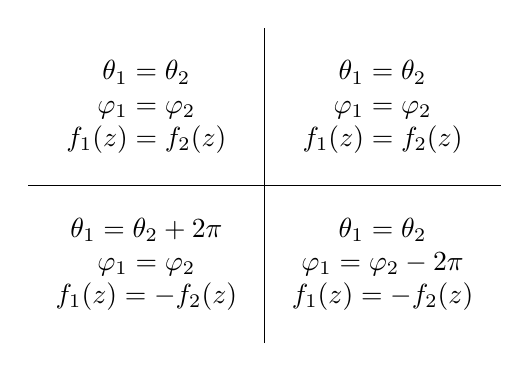
\begin{tikzpicture}
        \draw[black, thin] (-3,0) -- (3,0) ;
        \draw[black, thin] (0,-2) -- (0,2) ;
        \node[align=center] at (1.5,1) {$\theta_1=\theta_2$\\$\varphi_1=\varphi_2$\\$f_1(z)=f_2(z)$} ;
        \node[align=center] at (-1.5,1) {$\theta_1=\theta_2$\\$\varphi_1=\varphi_2$\\$f_1(z)=f_2(z)$} ;
        \node[align=center] at (-1.5,-1) {$\theta_1=\theta_2+2\pi$\\$\varphi_1=\varphi_2$\\$f_1(z)=-f_2(z)$} ;
        \node[align=center] at (1.5,-1) {$\theta_1=\theta_2$\\$\varphi_1=\varphi_2-2\pi$\\$f_1(z)=-f_2(z)$} ;
    \end{tikzpicture}
\end{center}
So the two cases have the same values in the upper half-plane, and with opposite signs in the lower half-plane.

\paragraph{11.6.5}
\begin{center}
    \begin{tabular}{>{\centering\arraybackslash}p{1.5cm} >{\centering\arraybackslash}p{2cm} >{\centering\arraybackslash}p{1.5cm}}
    \hline
    Point & Type & Order \\
    \hline
    $0$ & branch point & $12$ \\
    $2$ & branch point & $2$ \\
    $3$ & pole & $3$  \\
    $\infty$ & branch point & $12$ 
    \end{tabular}
\end{center}
where $12$ comes from the least common multiple of $3$ and $4$, and the property at infinity is identified by substituting $z=t^{-1}$:
\[
t^{\frac{1}{3}}+t^{\frac{1}{4}}(1-3t)^{-3}\,t^{3}+(1-2t)^{\frac{1}{2}}\,t^{-\frac{1}{2}}
\]

\paragraph{11.6.6}
\[
F(z)=\ln(z+i)+\ln(z-i)
\]
\[
F(i,-2)-F(0,0)=\ln(2\sqrt{2}e^{i\frac{\pi}{4}})+\ln(2e^{-i\frac{\pi}{2}})=\ln(4\sqrt{2})-i\frac{\pi}{4}
\]
so
\[
F(i,-2)=\ln(4\sqrt{2})-\frac{9i\pi}{4}
\]

\paragraph{11.6.7}
\[
-1=e^{(1+2n)i\pi}
\]
\[
\ln(-1)=(1+2n)i\pi
\]
where $n$ is an integer.

\paragraph{11.6.8}
At $z=0$, 
\[
\sum_{n=0}^\infty\binom{m}{n}z^n=1
\]
so the function $f(z)=(1+z)^m$ must take the branch in which $f(0)=1$. An appropriate branch cut is from $(-1,0)$ to $(-\infty,0)$, while all the branch cuts starting from $(-1,0)$ and lying in the left side of $x=-1$ are valid. If $|z|\geq1$, then it will contain a part of the branch cut and therefore result in discontinuity, while the expansion contains no discontinuity, so the domain must be restricted to $|z|<1$.

\paragraph{11.6.9}
If the branch of $f(z)=(1+z)^m$ at $z=0$ has the value
\[
\left[f(0)\right]_{branch\,N}=e^{m\cdot 2N\pi i}
\]
where $N$ is an integer, then at every point in the plane,
\[
\frac{\left[f(z)\right]_{branch\,N}}{\left[f(z)\right]_{branch\,0}}=e^{2mN\pi i}
\]
so the expansion becomes
\[
\left[(1+z)^m\right]_{branch\,N}=\sum_{z=0}^\infty e^{2mN\pi i}\binom{m}{n}z^n
\]

\paragraph{11.6.10}
(a)
\[
f(z)=\frac{1}{z-1}-\frac{1}{z}=\frac{1}{z-1}-\frac{1}{1+(z-1)}\]
\[=\frac{1}{z-1}-\sum_{n=0}^\infty(-1)^n(z-1)^n=\sum_{n=-1}^\infty(-1)^{n+1}(z-1)^n
\]
The expansion holds in the range $0<|z-1|<1$.
\medskip

(b)
\[
f(z)=\frac{1}{z-1}-\frac{1}{z}=\frac{1}{z-1}-\frac{1}{(z-1)}\frac{1}{1+(z-1)^{-1}}\]
\[=\frac{1}{z-1}-\frac{1}{z-1}\sum_{n=0}^\infty(-1)^n(z-1)^{-n}=\sum_{n=2}^\infty(-1)^n(z-1)^{-n}
\]
The expansion holds in the range $|z-1|>1$.

\paragraph{11.6.11}
(a) For $z=0$, 
\[
f_1(z)=\int_0^\infty dt=\infty
\]
For $z\neq0$,
\[
f_1(z)=\int_0^\infty e^{-zt}dt=\left[\frac{e^{-zt}}{-z} \right]_0^\infty=\frac{\left[e^{-zt}\right]_{t=\infty}-1}{-z}
\]
and note that
\[
\left[e^{-zt}\right]_{t=\infty}=
\begin{cases}
0,\qquad & \mathfrak{Re}(z)>0\\
\infty,\qquad & \mathfrak{Re}(z)<0
\end{cases}
\]
so the integral exists only for $\mathfrak{Re}(z)>0$.
\medskip

(b) For $\mathfrak{Re}(z)>0$,
\[
f_1(z)=\frac{0-1}{-z}=\frac{1}{z}
\]

(c)
\[
\frac{1}{z}=\frac{1}{-i+(z+i)}=\frac{1}{(-i)}\frac{1}{1+i(z+i)}
\]
\[
=i\sum_{n=0}^\infty(-1)^n\,i^n(z+i)^n\]
\[=i\sum_{n=0}^\infty i^{-n}(z+i)^n
\]
The expansion is valid in $|z+i|<1$.

\section*{11.7 Calculus of Residues}

\paragraph{11.7.1 }
(a)
\begin{alignat*}{3}
    & z=ia:\qquad && \textit{simple pole,}\qquad && a_{-1}=\lim_{z\to ia}\frac{(z-ia)}{z^2+a^2}=\lim_{z\to ia}\frac{1}{z+ia}=\frac{1}{2ia}\\
    & z=-ia:\qquad && \textit{simple pole,}\qquad && a_{-1}=\lim_{z\to -ia}\frac{(z+ia)}{z^2+a^2}=\lim_{z\to -ia}\frac{1}{z-ia}=-\frac{1}{2ia}\\
\end{alignat*}

(b)
\begin{alignat*}{3}
    & z=ia:\qquad && \textit{second-order pole,}\qquad && a_{-1}=\lim_{z\to ia}\left[\frac{d}{dz}\frac{(z-ia)^2}{(z^2+a^2)^2} \right]=\lim_{z\to ia}\left[\frac{-2}{(z+ia)^3} \right]=\frac{1}{4ia^3}\\
    & z=-ia:\qquad && \textit{second-order pole,}\qquad && a_{-1}=\lim_{z\to -ia}\left[\frac{d}{dz}\frac{(z+ia)^2}{(z^2+a^2)^2} \right]=\lim_{z\to -ia}\left[\frac{-2}{(z-ia)^3} \right]=-\frac{1}{4ia^3}
\end{alignat*}

(c)
\begin{alignat*}{3}
    & z=ia:\qquad && \textit{second-order pole,}\qquad && a_{-1}=\lim_{z\to ia}\left[\frac{d}{dz}\frac{z^2(z-ia)^2}{(z^2+a^2)^2} \right]=\lim_{z\to ia}\frac{-2}{(1+\frac{ia}{z})^3}\frac{-ia}{z^2}=\frac{1}{4ia}\\
    & z=-ia:\qquad && \textit{second-order pole,}\qquad && a_{-1}=\lim_{z\to -ia}\left[\frac{d}{dz}\frac{z^2(z+ia)^2}{(z^2+a^2)^2} \right]=\lim_{z\to -ia}\frac{-2}{(1-\frac{ia}{z})^3}\frac{ia}{z^2}=-\frac{1}{4ia}
\end{alignat*}

(d)
\begin{alignat*}{3}
    & z=0:\qquad && \textit{essential singularity,}\qquad && a_{-1}=\frac{\sinh(\frac{1}{a})}{a} \\
    & z=ia:\qquad && \textit{simple pole,}\qquad && a_{-1}=\lim_{z\to ia}\frac{(z-ia)\sin\frac{1}{z}}{z^2+a^2}=\lim_{z\to ia}\frac{\sin\frac{1}{z}}{z+ia}=\frac{-\sinh(\frac{1}{a})}{2a}\\
    & z=-ia:\qquad && \textit{simple pole,}\qquad && a_{-1}=\lim_{z\to -ia}\frac{(z+ia)\sin\frac{1}{z}}{z^2+a^2}=\lim_{z\to -ia}\frac{\sin\frac{1}{z}}{z-ia}=\frac{-\sinh(\frac{1}{a})}{2a}
\end{alignat*}

The residue at $z=0$ is obtained from the expansion:
\[
\frac{\sin(\frac{1}{z})}{z^2+a^2}=\left(\frac{1}{z}-\frac{1}{3!z^3}+\frac{1}{5!z^5}-\cdots \right)\frac{1}{a^2}\left(1-\frac{z^2}{a^2}+\frac{z^4}{a^4}-\cdots \right)
\]

The coefficient of $\frac{1}{z}$ is 
\[
a_{-1}=\frac{1}{a}\left(\frac{1}{a}+\frac{1}{3!a^3}+\frac{1}{5!a^5}+\cdots \right)=\frac{\sinh(\frac{1}{a})}{a}
\]

Note that the sum of all the residues is zero, which confirms our answer.
\medskip

(e)
\begin{alignat*}{3}
    & z=ia:\qquad && \textit{simple pole,}\qquad && a_{-1}=\lim_{z\to ia}\frac{(z-ia)ze^{iz}}{z^2+a^2}=\lim_{z\to ia}\frac{ze^{iz}}{z+ia}=\frac{e^{-a}}{2}\\
    & z=-ia:\qquad && \textit{simple pole,}\qquad && a_{-1}=\lim_{z\to -ia}\frac{(z+ia)ze^{iz}}{z^2+a^2}=\lim_{z\to -ia}\frac{ze^{iz}}{z-ia}=\frac{e^{a}}{2}\\
    & z=\infty:\qquad && \textit{essential singularity,}\qquad && a_{-1}=-\cosh a
\end{alignat*}

The residue at $z=\infty$ is obtained by substituting $z=\frac{1}{w}$,\; $f(z)=g(w)$ and note that
\[
\oint\displaylimits_Cf(z)dz=\oint\displaylimits_C-g(w)\frac{dw}{w^2}
\]

so the residue of $f(z)$ at $\infty$ is the residue of $-\frac{g(w)}{w^2}$ at $0$. From the expansion,
\[
-\frac{g(w)}{w^2}=
-\frac{1}{w^2}\frac{\frac{1}{w}e^{i\frac{1}{w}}}{\frac{1}{w^2}+a^2}=-\frac{1}{w}\left(1+\frac{i}{w}+\frac{-1}{2!w^2}+\frac{-i}{3!w^3}+\cdots \right)\left(1-a^2w^2+a^4w^4-\cdots \right)
\]

The coefficient of $\frac{1}{w}$ is 
\[
a_{-1}=-\left(1+\frac{a^2}{2!}+\frac{a^4}{4!}+\cdots \right)=-\cosh a
\]

Note that the sum of all the residues is zero, which confirms our answer.
\medskip

(f)
\begin{alignat*}{3}
    & z=a:\qquad && \textit{simple pole,}\qquad && a_{-1}=\lim_{z\to a}\frac{(z-a)ze^{iz}}{z^2-a^2}=\lim_{z\to a}\frac{ze^{iz}}{z+a}=\frac{e^{ia}}{2}\\
    & z=-a:\qquad && \textit{simple pole,}\qquad && a_{-1}=\lim_{z\to -a}\frac{(z+a)ze^{iz}}{z^2-a^2}=\lim_{z\to -a}\frac{ze^{iz}}{z-a}=\frac{e^{-ia}}{2}\\
    & z=\infty:\qquad && \textit{essential singularity,}\qquad && a_{-1}=-\cos a
\end{alignat*}

The residue at $\infty$ is obtained from the expansion:
\[
-\frac{g(w)}{w^2}=
-\frac{1}{w^2}\frac{\frac{1}{w}e^{i\frac{1}{w}}}{\frac{1}{w^2}-a^2}=-\frac{1}{w}\left(1+\frac{i}{w}+\frac{-1}{2!w^2}+\frac{-i}{3!w^3}+\cdots \right)\left(1+a^2w^2+a^4w^4+\cdots \right)
\]

The coefficient of $\frac{1}{w}$ is 
\[
a_{-1}=-\left(1-\frac{a^2}{2!}+\frac{a^4}{4!}-\cdots \right)=-\cos a
\]

Note that the sum of all the residues is zero, which confirms our answer.
\medskip

(g)
\begin{alignat*}{3}
    & z=a:\qquad && \textit{simple pole,}\qquad && a_{-1}=\lim_{z\to a}\frac{(z-a)e^{iz}}{z^2-a^2}=\lim_{z\to a}\frac{e^{iz}}{z+a}=\frac{e^{ia}}{2a}\\
    & z=-a:\qquad && \textit{simple pole,}\qquad && a_{-1}=\lim_{z\to -a}\frac{(z+a)e^{iz}}{z^2-a^2}=\lim_{z\to -a}\frac{e^{iz}}{z-a}=-\frac{e^{-ia}}{2a}\\
    & z=\infty:\qquad && \textit{essential singularity,}\qquad && a_{-1}=-\frac{i\sin a}{a}
\end{alignat*}

The residue at $\infty$ is obtained from the expansion:
\[
-\frac{g(w)}{w^2}=
-\frac{1}{w^2}\frac{e^{i\frac{1}{w}}}{\frac{1}{w^2}-a^2}=-\left(1+\frac{i}{w}+\frac{-1}{2!w^2}+\frac{-i}{3!w^3}+\cdots \right)\left(1+a^2w^2+a^4w^4+\cdots \right)
\]

The coefficient of $\frac{1}{w}$ is 
\[
a_{-1}=-\frac{i}{a}\left(a-\frac{a^3}{3!}+\frac{a^5}{5!}-\cdots \right)=-\frac{i\sin a}{a}
\]

Note that the sum of all the residues is zero, which confirms our answer.
\medskip

(h)
\begin{alignat*}{3}
    & z=-1:\qquad && \textit{simple pole,}\qquad && a_{-1}=\lim_{z\to-1}\frac{(z+1)z^{-k}}{z+1}=(-1)^{-k}\\
    & z=0:\qquad && \textit{branch point,} && 
\end{alignat*}

\paragraph{11.7.2}
\begin{alignat*}{2}
    & z=0:\qquad && \frac{\pi\cot\pi z}{z(z+1)}=\frac{\pi\frac{\cos\pi z}{\sin\pi z}}{z(z+1)}=\pi\frac{1-\frac{(\pi z)^2}{2!}+\cdots}{\pi z-\frac{(\pi z)^3}{3!}+\cdots}\cdot\frac{1-z+z^2-\cdots}{z}=\frac{1}{z^2}-\frac{1}{z}+\sum_{n=0}^\infty a_nz^n\\
    & z=1:\qquad && \frac{\pi\cot\pi z}{z(z+1)}=\frac{\pi\cot\pi t}{(t-1)t}=\pi\frac{1-\frac{(\pi t)^2}{2!}+\cdots}{\pi t-\frac{(\pi t)^3}{3!}+\cdots}\cdot\frac{-(1+t+t^2+\cdots)}{t}=-\frac{1}{t^2}-\frac{1}{t}+\sum_{n=0}^\infty b_n t^n
\end{alignat*}
where we substitute $t$ for $z+1$ in the second equation, so both the residues at $z=0$ and $z=-1$ are  equals to $-1$.

\paragraph{11.7.3}
\[
\dashint_{-\infty}^x\frac{e^t}{t}dt=
\lim_{\delta\to0}\left[\int_{-\infty}^{-\delta}\frac{e^t}{t}dt+\int_{\delta}^x\frac{e^t}{t}dt \right]\]
\[
=\lim_{\delta\to0}\left[-\int_{\delta}^{\infty}\frac{e^{-t}}{t}dt+\int_{\delta}^x\frac{e^t}{t}dt
 \right]\]
\[ =\lim_{\delta\to0}\left[\int_{\delta}^x\frac{e^t-e^{-t}}{t}dt+\int_x^\infty\frac{e^{-t}}{t}dt \right]
\]
where the first integral exists because $\frac{e^t-e^{-t}}{t}$ is finite as  $t\to0$, and the second integral exists because $\int_x^\infty e^{-t}dt$ is finite.



\paragraph{11.7.4}
\[
\dashint_0^\infty\frac{x^{-p}}{x-1}dx=\lim_{\delta\to0}\left[\int_0^{1-\delta}\frac{x^{-p}}{x-1}dx+\int_{1+\delta}^\infty\frac{x^{-p}}{x-1}dx \right]
\]
\[
=\lim_{\delta\to0}\left[-\int_0^{1-\delta}x^{-p}\sum_{n=0}^\infty x^ndx+\int_{1+\delta}^\infty x^{-p}x^{-1}\sum_{n=0}^\infty x^{-n}dx \right]
\]
\[
=\lim_{\delta\to0}\left[-\sum_{n=0}^\infty\frac{(1-\delta)^{-p+n+1}}{-p+n+1}+\sum_{n=0}^\infty\frac{-(1+\delta)^{-p-n}}{-p-n} \right]
\]
\[
=\sum_{n=0}^\infty\frac{1}{p-n-1}+\sum_{n=0}^\infty\frac{1}{p+n}
\]
\[
=\frac{1}{p}+\sum_{n=1}^\infty\frac{2p}{p^2-n^2}=\pi\cot \pi p
\]
where we use Equation 11.81 in the last equation:
\[
\cot \pi p=\frac{1}{\pi p}+2\pi p\sum_{n=1}^\infty\frac{1}{\pi^2p^2-\pi^2n^2}=\frac{1}{\pi}\left(\frac{1}{p}+\sum_{n=1}^\infty\frac{2p}{p^2-n^2} \right)
\]

\paragraph{11.7.5}
The conditions for Equation 1.88 to hold is that $f(z)$ being an entire function, and $\frac{f'(z)}{f(z)}$ being analytic at $z=0$. If $f(z)=\sin x$, then $\left[\frac{f'(z)}{f(z)}\right]_{z\to0}=\left[\frac{\cos z}{\sin z}\right]_{z\to0}=\infty$, which does not meet the second condition. If $f(z)=\frac{\sin z}{z}$, then $\left[\frac{\sin z}{z}\right]_{z\to0}=1$, so $f(z)$ is an entire function, and \[
\lim_{z\to0}\frac{f'(z)}{f(z)}=\lim_{z\to0}\frac{\frac{\cos z}{z}-\frac{\sin z}{z^2}}{\frac{\sin z}{z}}=\lim_{z\to0}\frac{(\frac{1}{z}-\frac{z}{2!}+\cdots)-(\frac{1}{z}-\frac{z}{3!}+\cdots)}{1-\frac{z^2}{3!}+\cdots}=\lim_{z\to0}\frac{-\frac{1}{6}z+\cdots}{1+\cdots}=0
\]
so $\frac{f'(z)}{f(z)}$ is analytic at $0$. Then we can use Equation 11.88, and note that the zeros of $f(z)$ is $z_n=n\pi$ for all positive and negative integers except for $0$:
\[
\frac{\sin z}{z}=1\cdot e^{0}\cdot \prod_{\substack{n=-\infty\\n\neq0}}^\infty\left(1-\frac{z}{n\pi}\right)e^{\frac{z}{n\pi}}\]
\[=\prod_{n=1}^\infty\left(1-\frac{z}{n\pi}\right)e^{\frac{z}{n\pi}}\left(1+\frac{z}{n\pi}\right)e^{-\frac{z}{n\pi}}
\]
\[
=\prod_{n=1}^\infty\left(1-\frac{z^2}{n^2\pi^2}\right)
\]
so
\[
\sin z=z\prod_{n=1}^\infty\left(1-\frac{z^2}{n^2\pi^2}\right)
\]

\paragraph{11.7.6}
For a polynomial $\sum_{k=1}^n a_kz^k$, let $f(z)=a_nz^n$, and $g(z)=\sum_{k=1}^{n-1}a_kz^k$. On the contour of radius $R$ which is sufficiently large, we have $|f(z)|>|g(z)|$, so by Rouché’s theorem, the polynomial which is $f(z)+g(z)$, has the same number of zeros with $f(z)$, which is $n$. 

\paragraph{11.7.7}
First consider the contour $|z|=1$, and let $f(z)=10$, $g(z)=z^6-4z^3$ (more precisely the radius should be $\lim_{\delta\to0^+}(1-\delta)$ to eliminate the zero on $|z|=1$). Because $|f(z)|>|g(z)|$ on $|z|=1$, by Rouché’s theorem, $z^6-4z^3+10=f(z)+g(z)$ has the same number of zeros with $f(z)$, which is no zero.

Then consider the contour $|z|=2$, and let $f(z)=z^6$, $g(z)=-4z^3+10$. Because $|f(z)|>|g(z)|$ on $|z|=2$, by Rouché’s theorem, $z^6-4z^3+10=f(z)+g(z)$ has the same number of zeros with $f(z)$, which is six zeros. By the fundamental theorem of algebra, $z^6-4z^3+10$ has six zeros, so all the zeros lie between $|z|=1$ and $|z|=2$.

\paragraph{11.7.8}
$\sec(0)=1$, so the Mittag-Leffler’s theorem is applicable. The poles of $\sec z$ are $z_n=\pm\frac{(2n+1)\pi}{2}$, $n$ is integer from $0$ to $\infty$. The residues are:
\[
b_n=\lim_{z\to\pm\frac{(2n+1)\pi}{2}}\frac{z\mp\frac{(2n+1)\pi}{2}}{\cos z}=\frac{1}{-\sin z}\Big|_{z=\pm\frac{(2n+1)\pi}{2}}=\mp(-1)^n
\]
so
\[
\sec z=1-\sum_{n=0}^\infty(-1)^n\left(\frac{1}{z-\frac{(2n+1)\pi}{2}}+\frac{1}{\frac{(2n+1)\pi}{2}} \right)+\sum_{n=0}^\infty(-1)^n\left(\frac{1}{z+\frac{(2n+1)\pi}{2}}+\frac{1}{-\frac{(2n+1)\pi}{2}} \right)
\]
\[
=\sum_{n=0}^\infty(-1)^n\frac{(2n+1)\pi}{\left(\frac{2n+1}{2}\right)^2\pi^2-z^2}+1-\frac{4}{\pi}\sum_{n=0}^\infty(-1)^n\frac{1}{2n+1}
\]
\[
=\pi\left(\frac{1}{(\frac{\pi}{2})^2-z^2}-\frac{3}{(\frac{3\pi}{2})^2-z^2}+\frac{5}{(\frac{5\pi}{2})^2-z^2}-\cdots \right)
\]
Note that 
\[
1-\frac{4}{\pi}\sum_{n=0}^\infty(-1)^n\frac{1}{2n+1}=1-\frac{4}{\pi}\cdot\frac{\pi}{4}=0
\]
from the results of Exercise 1.3.2.
\medskip

Let $f(z)=\csc z-\frac{1}{z}$, then
\[
\lim_{z\to0}f(z)=\lim_{z\to0}\left[\frac{1}{z}+\frac{z}{3!}+\cdots-\frac{1}{z} \right]=0
\]
so $f(z)$ is analytic at $z=0$. The poles of $f(z)$ are $z_n=\pm n\pi$, where $n\neq0$. The residues are:
\[
b_n=\lim_{z\to\pm n\pi}\frac{z\mp n\pi}{\sin z}=\lim_{z\to\pm n\pi}\frac{1}{\cos z}=(-1)^n
\]
so
\[
\csc z-\frac{1}{z}=\sum_{n=1}^\infty(-1)^n\left(\frac{1}{z-n\pi}+\frac{1}{n\pi} \right)+\sum_{n=1}^\infty(-1)^n\left(\frac{1}{z+n\pi}+\frac{1}{-n\pi} \right)
\]
\[
=\sum_{n=1}^\infty(-1)^n\frac{2z}{z^2-n^2\pi^2}
\]
so
\[
\csc z=\frac{1}{z}+\sum_{n=1}^\infty(-1)^n\frac{2z}{z^2-n^2\pi^2}
\]
\[
=\frac{1}{z}-2z\left(\frac{1}{z^2-\pi^2}-\frac{1}{z^2-(2\pi)^2}+\frac{1}{z^2-(3\pi)^2}-\cdots \right)
\]

\paragraph{11.7.9}
$f(z)=(z-1)(z-2)z^{-1}$, so it has two zeros at $1,2$, and a simple pole at $0$. Differentiate, 
\[
f'(z)=(z-2)z^{-1}+(z-1)z^{-1}-(z-1)(z-2)z^{-2}
\]
\[
\frac{f'(z)}{f(z)}=\frac{1}{z-1}+\frac{1}{z-2}-\frac{1}{z}
\]
so it is clear that if a contour $C$ encircle $N_f$ zeros and $P_f$ poles (the multiplicity and order of all the zeros and poles are $1$), then
\[
\oint\displaylimits_C\frac{f'(z)}{f(z)}dz=2\pi i(N_f-P_f)
\]

\paragraph{11.7.10}
Let $z=e^{i\theta}$, then $dz=e^{i\theta}d\theta$, and
\[
\int\displaylimits_{\substack{|z|=1\\semicircle}}z^{-2}dz=\int\displaylimits_0^\pi e^{-2i\theta}e^{i\theta}d\theta=\left[ie^{-i\theta} \right]_0^\pi=-2i
\]
but
\[
\oint\displaylimits_{|z|=1}z^{-2}dz=0
\]
so the equation does not necessary hold for poles of higher order.

\paragraph{11.7.11}
(a)
\[
\lim_{\delta\to0}\left[\int_{-\infty}^{x_0-\delta}\frac{a_{-3}}{(x-x_0)^3}dx+\int_{x_0+\delta}^\infty\frac{a_{-3}}{(x-x_0)^3}dx \right]
\]
\[
=\lim_{\delta\to0}\left[\frac{a_{-3}}{-2(x-x_0)^2}\Big|_{-\infty}^{x_0-\delta}+\frac{a_{-3}}{-2(x-x_0)^2}\Big|_{x_0+\delta}^\infty \right]
\]
\[
=\lim_{\delta\to0}\left[\frac{a_{-3}}{-2\delta^2}-\frac{a_{-3}}{-2\delta^2}\right]=0
\]
so the integration of $\frac{a_{-3}}{(x-x_0)^3}$ is cancelled out.
\[
\lim_{\delta\to0}\left[\int_{-\infty}^{x_0-\delta}\frac{a_{-1}}{x-x_0}dx+\int_{x_0+\delta}^\infty\frac{a_{-1}}{x-x_0}dx \right]
\]
\[
=\lim_{\delta\to0}\left[a_{-1}\ln(x-x_0)\Big|_{-\infty}^{x_0-\delta}+a_{-1}\ln(x-x_0)\Big|_{x_0+\delta}^\infty \right]
\]
\[
=\lim_{\delta\to0}\left[a_{-1}\ln\frac{-\delta\cdot\infty}{-\infty\cdot\delta} \right]=0
\]
so the integration of $\frac{a_{-1}}{x-x_0}$ is cancelled out. $g(z)$ is analytic along the whole real axis, so the Cauchy principle value is finite.
\medskip

(b)
Let $z-z_0=re^{i\theta}$, $dz=ire^{i\theta}d\theta$, then
\[
I_{over}=\int_\pi^0\left[\frac{a_{-3}}{r^3e^{3i\theta}}+\frac{a_{-1}}{re^{i\theta}}+a_0+\cdots \right]ire^{i\theta}d\theta
\]
\[
=\int_\pi^0\left(\frac{ia_{-3}}{r^2e^{2i\theta}}+ia_{-1}+ire^{i\theta}a_0+\cdots \right)d\theta
\]
\[
=\left[\frac{a_{-3}}{-2r^2}e^{-2i\theta}+ia_{-1}\theta+re^{i\theta}a_0+\cdots \right]_\pi^0
\]
\[
=-i\pi a_{-1},\qquad\textit{when $r\to0$}
\]
similarly,
\[
I_{under}=\left[\frac{a_{-3}}{-2r^2}e^{-2i\theta}+ia_{-1}\theta+re^{i\theta}a_0+\cdots \right]_\pi^{2\pi}
\]
\[
=i\pi a_{-1},\qquad\textit{when $r\to0$}
\]

\paragraph{11.7.12}
(The problem requires techniques from the next section, especially Equation 11.102)
\medskip

(a) (The integral should be a normal integral, not a Cauchy principle value.) The function $\frac{e^{izs}}{z-i\varepsilon}$ has a simple pole at $z=i\varepsilon$ with residue $e^{-\varepsilon s}$. For $\varepsilon\to0^+$, the pole is in the upper half-plane, and the residue is $\lim_{\varepsilon\to0}e^{-\varepsilon s}=1$.

For $s<0$, let the contour be a semicircle in the lower half-plane, with the radius $R\to\infty$. Then
\[
\oint\displaylimits_C\frac{e^{izs}}{z-i\varepsilon}dx=\int\displaylimits_{-\infty}^\infty\frac{e^{ixs}}{x-i\varepsilon}dx+\int\displaylimits_{C_R}\frac{e^{izs}}{z-i\varepsilon}dz=0
\]
Because $\lim_{|z|\to\infty}\frac{e^{izs}}{z-i\varepsilon}=0$ in the lower half-plane, so $\int_{C_R}\frac{e^{izs}}{z-i\varepsilon}dz=0$ by Equation 11.102. Therefore, 
\[
\int_{-\infty}^\infty\frac{e^{ixs}}{x-i\varepsilon}dx=0
\]
and 
\[
u(s)=\frac{1}{2\pi i}\int_{-\infty}^\infty\frac{e^{ixs}}{x-i\varepsilon}dx=0,\qquad\textit{for $s<0$}
\]

For $s>0$, let the contour be a semicircle in the upper half-plane, with the radius $R\to\infty$. Then
\[
\oint\displaylimits_C\frac{e^{izs}}{z-i\varepsilon}dz=\int\displaylimits_{-\infty}^\infty\frac{e^{ixs}}{x-i\varepsilon}dx+\int\displaylimits_{C_R}\frac{e^{izs}}{z-i\varepsilon}dz=2\pi i
\]
Because $\lim_{|z|\to\infty}\frac{e^{izs}}{z-i\varepsilon}=0$ in the upper half-plane, so $\int_{C_R}\frac{e^{izs}}{z-i\varepsilon}dz=0$ by Equation 11.102. Therefore,
\[
\int_{-\infty}^\infty\frac{e^{ixs}}{x-i\varepsilon}dx=2\pi i
\]
and
\[
u(s)=\frac{1}{2\pi i}\int_{-\infty}^\infty\frac{e^{ixs}}{x-i\varepsilon}dx=1\qquad\textit{for $s>0$}
\]

(b)
The function $\frac{e^{izs}}{z}$ has a simple pole at $z=0$ with residue $1$.
For $s<0$, let the contour be a semicircle in the lower half-plane with radius $R\to\infty$, and circumvent $z=0$ by another semicircle with radius $r\to0$. Then
\[
\oint\displaylimits_C\frac{e^{izs}}{z}dz=\dashint_{-\infty}^\infty\frac{e^{ixs}}{x}dx+\int\displaylimits_{C_r}\frac{e^{izs}}{z}dz+\int\displaylimits_{C_R}\frac{e^{izs}}{z}dz=0
\]
Because $\lim_{|z|\to\infty}\frac{e^{izs}}{z}=0$ in the lower half-plane, so $\int_{C_R}\frac{e^{izs}}{z}dz=0$ by Equation 11.102. Because $\frac{e^{izs}}{z}$ has a simple pole at $z=0$ with residue $1$, so $\int_{C_r}\frac{e^{izs}}{z}dz=\pi i$ by Equation 11.76. Therefore,
\[
\dashint_{-\infty}^\infty\frac{e^{ixs}}{x}dx=-\pi i
\]
and
\[
u(s)=\frac{1}{2}+\frac{1}{2\pi i}\dashint_{-\infty}^\infty\frac{e^{ixs}}{x}dx=0\qquad\textit{for $s<0$}
\]

For $s>0$, let the contour be a semicircle in the upper half-plane with radius $R\to\infty$, and circumvent $z=0$ by another semicircle with radius $r\to0$. Then
\[
\oint\displaylimits_C\frac{e^{izs}}{z}dz=\dashint_{-\infty}^\infty\frac{e^{ixs}}{x}dx+\int\displaylimits_{C_r}\frac{e^{izs}}{z}dz+\int\displaylimits_{C_R}\frac{e^{izs}}{z}dz=0
\]
Because $\lim_{|z|\to\infty}\frac{e^{izs}}{z}=0$ in the upper half-plane, so $\int_{C_R}\frac{e^{izs}}{z}dz=0$ by Equation 11.102. Because $\frac{e^{izs}}{z}$ has a simple pole at $z=0$ with residue $1$, so $\int_{C_r}\frac{e^{izs}}{z}dz=-\pi i$ by Equation 11.75. Therefore,
\[
\dashint_{-\infty}^\infty\frac{e^{ixs}}{x}dx=\pi i
\]
and
\[
u(s)=\frac{1}{2}+\frac{1}{2\pi i}\dashint_{-\infty}^\infty\frac{e^{ixs}}{x}dx=1\qquad\textit{for $s>0$}
\]

\section*{11.8 Evaluation of Definite Integrals}

\paragraph{11.8.1}
Let $z=e^{i\theta}$, then $dz=ie^{i\theta}d\theta=izd\theta$. and
\[
\int\displaylimits_{0}^{2\pi}\frac{d\theta}{a+b\cos\theta}=\oint\displaylimits_{|z|=1}\frac{-iz^{-1}dz}{a+b\cdot\frac{z+z^{-1}}{2}}=\frac{-2i}{b}\oint\displaylimits_{|z|=1}\frac{dz}{z^2+\frac{2a}{b}z+1}=\frac{-2i}{b}\oint\displaylimits_{|z|=1}\frac{dz}{(z-\alpha)(z-\beta)}
\]
Note that $\alpha\beta=1$ and $\alpha\neq\beta$, so only one of the roots is in the unit circle, without loss of generality let it be $\alpha$. Then the residue at $z=\alpha$ is
\[
residue=\frac{1}{\alpha-\beta}=\frac{1}{\sqrt{(\alpha+\beta)^2-4\alpha\beta}}=\frac{1}{\sqrt{(-\frac{2a}{b})^2-4}}=\frac{b}{2\sqrt{a^2-b^2}}
\]
So the integral is
\[
I=\frac{-2i}{b}\cdot2\pi i\cdot\frac{b}{2\sqrt{a^2-b^2}}=\frac{2\pi}{\sqrt{a^2-b^2}}
\]
Note that replacing $b$ with $-b$ will not change the result.
\medskip

For the case of $\sin\theta$, let $\theta=\theta'+\frac{\pi}{2}$, then $d\theta=d\theta'$, and $\sin\theta=\cos\theta'$, so
\[
\int\displaylimits_0^{2\pi}\frac{d\theta}{a+b\sin\theta}=\int\displaylimits_{-\frac{\pi}{2}}^{\frac{3\pi}{2}}\frac{d\theta'}{a+b\cos\theta'}=\int\displaylimits_{0}^{2\pi}\frac{d\theta'}{a+b\cos\theta'}=\frac{2\pi}{\sqrt{a^2-b^2}}
\]
Note that because $\cos\theta$ is periodic, the integral will not change as long at the range of integration is $2\pi$.
\smallskip

If $|b|>|a|$, then there will be a singularity at $\theta=\cos^{-1}\pm\frac{a}{b}$ or $\theta=\sin^{-1}\pm\frac{a}{b}$, and therefore the integral does not exists.

\paragraph{11.8.2}
From Exercise 11.8.1, 
\[
\int\displaylimits_0^{2\pi}\frac{d\theta}{a+\cos\theta}=\frac{2\pi}{(a^2-1)^{\frac{1}{2}}}
\]
Differentiate with respect to $a$, we have
\[
\int\displaylimits_0^{2\pi}\frac{-d\theta}{(a+\cos\theta)^2}=\frac{-2\pi a}{(a^2-1)^{\frac{3}{2}}}
\]
so
\[
\int\displaylimits_0^{\pi}\frac{d\theta}{(a+\cos\theta)^2}=\frac{1}{2}\cdot\int\displaylimits_0^{2\pi}\frac{d\theta}{(a+\cos\theta)^2}=\frac{\pi a}{(a^2-1)^{\frac{3}{2}}}
\]

\paragraph{11.8.3}
For $|t|<1$, we have $1+t^2>|2t|$, so we can use the results from Exercise 11.8.1:
\[
\int\displaylimits_0^{2\pi}\frac{d\theta}{(1+t^2)-2t\cos\theta}=\frac{2\pi}{\sqrt{(1+t^2)^2-(2t)^2}}=\frac{2\pi}{1-t^2}
\]
For $|t|>1$, we still have $1+t^2>|2t|$, but the integral becomes
\[
\int\displaylimits_0^{2\pi}\frac{d\theta}{(1+t^2)-2t\cos\theta}=\frac{2\pi}{\sqrt{(1+t^2)^2-(2t)^2}}=\frac{2\pi}{t^2-1}
\]
For $|t|=1$, there will be a singularity at $\theta=0$ or $\theta=\pi$, and therefore the integral does not exists.

\paragraph{11.8.4}
Let $z=e^{i\theta}$, then
\[
\int\displaylimits_0^{2\pi}\frac{\cos3\theta\,d\theta}{5-4\cos\theta}=\oint\displaylimits_{|z|=1}\frac{\frac{z^3+z^{-3}}{2}\cdot(-iz^{-1}dz)}{5-4\frac{z+z^{-1}}{2}}=\frac{i}{2}\oint\displaylimits_{|z|=1}\frac{(z^6+1)}{z^3(2z-1)(z-2)}dz
\]
The function has a third pole at $z=0$ and a simple pole at $z=\frac{1}{2}$ in the unit circle. The residue of $z=0$ is easier to obtained from the expansion:
\[
\frac{(1+z^6)(1+2z+4z^2+\cdots)(1+\frac{z}{2}+\frac{z^2}{4}+\cdots)}{2z^3}=\frac{1}{2}z^{-3}+\frac{5}{4}z^{-2}+\frac{21}{8}z^{-1}+\cdots
\]
so
\[
residue_{z=0}=\frac{21}{8}
\]
The residue at $z=\frac{1}{2}$ is
\[
residue_{z=\frac{1}{2}}=\frac{\frac{1}{64}+1}{\frac{1}{8}\cdot2\cdot(\frac{1}{2}-2)}=-\frac{65}{24}
\]
so the integral is
\[
I=\frac{i}{2}\cdot2\pi i\cdot(\frac{21}{8}-\frac{65}{24})=\frac{\pi}{12}
\]

\paragraph{11.8.5}
\[
\int\displaylimits_0^\pi\cos^{2n}\theta\,d\theta=\frac{1}{2}\int\displaylimits_0^{2\pi}\cos^{2n}\theta\,d\theta
\]
\[
=\frac{1}{2}\oint\displaylimits_{|z|=1}\left(\frac{z+z^{-1}}{2} \right)^{2n}\cdot(-iz^{-1}dz)
\]
\[
=\frac{-i}{2}\oint\displaylimits_{|z|=1}\frac{z^{-1}dz}{2^{2n}}\sum_{k=0}^{2n}\binom{2n}{k}z^{2n-2k}
\]
\[
=\frac{-i}{2}\oint\displaylimits_{|z|=1}\left[\frac{1}{2^{2n}}\binom{2n}{n}z^{-1}+\sum_{k\neq-1}a_kz^k \right]dz
\]
\[
=\frac{-i}{2}\cdot2\pi i\cdot\frac{1}{2^{2n}}\cdot\frac{(2n)!}{n!\cdot n!}
\]
\[
=\pi\frac{(2n)!}{2^{2n}(n!)^2}=\pi\frac{(2n-1)!!}{(2n)!!}
\]

\paragraph{11.8.6}
\[
\left(1-e^{\frac{2\pi i}{3}}\right)I-\frac{2\pi i}{3}e^{\frac{2\pi i}{3}}\left(\frac{2\pi}{3\sqrt{3}}\right)=(2\pi i)\left(\frac{\pi i}{9}\right)e^{-\frac{2\pi i}{3}}
\]
\[
\left(1+\frac{1}{2}-\frac{\sqrt{3}i}{2}\right)I=\frac{4\pi^2i}{9\sqrt{3}}\left(-\frac{1}{2}+\frac{\sqrt{3}i}{2}\right)-\frac{2\pi^2}{9}\left(-\frac{1}{2}-\frac{\sqrt{3}i}{2}\right)
\]
\[
\left(\frac{3}{2}-\frac{\sqrt{3}i}{2}\right)I=-\frac{\pi^2}{9}+\frac{\sqrt{3}\pi^2i}{27}
\]
\[
\sqrt{3}e^{-\frac{\pi i}{6}}I=\frac{2\sqrt{3}\pi^2}{27}e^{\frac{5\pi i}{6}}
\]
\[
I=-\frac{2\pi^2}{27}
\]

\paragraph{11.8.7}
The integral on small circle vanishes because
\[
\lim_{r\to0}\int_{C_r}\frac{z^pdz}{z^2+1}=
\lim_{r\to0}\int_{2\pi}^0\frac{r^pe^{ip\theta}(ire^{i\theta }d\theta)}{r^2e^{2i\theta}+1}=\lim_{r\to0}\int_{2\pi}^0 r^{1+p}\frac{ie^{i(p+1)\theta}}{1+r^2e^{2i\theta}}d\theta=0
\]
The integral on large circle vanishes because
\[
\lim\displaylimits_{|z|\to\infty}z\cdot\frac{z^p}{z^2+1}=\lim_{|z|\to\infty }z^{p-1}=\lim_{|z|\to\infty}\frac{1}{z^{1-p}}=0
\]
so from Equation 11.96,
\[
\lim_{R\to\infty}\int_{C_R}\frac{z^pdz}{z^2+1}=0
\]
Simplifying Equation 11.115:
\[
\left(1-e^{2p\pi i}\right)I=(2\pi i)\frac{1}{2i}\left(e^{\frac{p\pi i}{2}}-e^{\frac{3p\pi i}{2}} \right)
\]
\[
\left(e^{-p\pi i}-e^{p\pi i} \right)I=\pi\left(e^{-\frac{p\pi i}{2}-}e^{\frac{p\pi i}{2}} \right)
\]
\[
I=\frac{\pi\cdot(-2i)\sin(\frac{p\pi}{2})}{(-2i)\sin(p\pi)}=\frac{\pi\sin(\frac{p\pi}{2})}{\sin(p\pi)}=\frac{\pi}{2\cos(\frac{p\pi}{2})}
\]

\paragraph{11.8.8}
\[
\int\displaylimits_{-\infty}^\infty\frac{\cos bx-\cos ax}{x^2}dx=\int\displaylimits_{-\infty}^\infty\frac{(e^{ibx}+e^{-ibx})-(e^{iax}-e^{-iax})}{2x^2}dx=\ddashint\displaylimits_{-\infty}^\infty\frac{e^{ibx}-e^{iax}}{2x^2}dx+\ddashint\displaylimits_{-\infty}^\infty\frac{e^{-ibx}-e^{-iax}}{2x^2}dx
\]
For the first integral, the function has a simple pole at $z=0$ with residue
\[
\lim_{z\to0}z\cdot\frac{e^{ibz}-e^{iaz}}{2z^2}=\lim_{z\to0}\frac{ib\,e^{ibz}-ia\,e^{iaz}}{2}=\frac{i(b-a)}{2}
\]
and Equation 11.102 is applicable because the function vanishes when $|z|\to\infty$. Take the contour to be the semicircle with $R\to\infty$ in the upper half-plane, then
\[
\oint\frac{e^{ibz}-e^{iaz}}{2z^2}dz=\ddashint\displaylimits_{-\infty}^\infty\frac{e^{ibx}-e^{iax}}{2x^2}dx+\int\displaylimits_{C_r}\frac{e^{ibz}-e^{iaz}}{2z^2}dz+\int\displaylimits_{C_R}\frac{e^{ibz}-e^{iaz}}{2z^2}dz
\]
\[
=\ddashint\displaylimits_{-\infty}^\infty\frac{e^{ibx}-e^{iax}}{2x^2}dx-\frac{2\pi i}{2}\cdot\frac{i(b-a)}{2}+0=0
\]
so
\[
\ddashint\displaylimits_{-\infty}^\infty\frac{e^{ibx}-e^{iax}}{2x^2}dx=\frac{\pi(a-b)}{2}
\]
Similarly, for the second integral, the function has a simple pole at $z=0$ with residue
\[
\lim_{z\to0}z\cdot\frac{e^{-ibz}-e^{-iaz}}{2z^2}=\lim_{z\to0}\frac{-ib\,e^{-ibz}+ia\,e^{-iaz}}{2}=\frac{i(a-b)}{2}
\]
and the lower half-plane version of Equation 11.102 is applicable because the function vanishes when $|z|\to\infty$. Take the contour to be the semicircle with $R\to\infty$ in the lower half-plane, then
\[
\oint\frac{e^{-ibz}-e^{-iaz}}{2z^2}dz=\ddashint\displaylimits_{-\infty}^\infty\frac{e^{-ibx}-e^{-iax}}{2x^2}dx+\int\displaylimits_{C_r}\frac{e^{-ibz}-e^{-iaz}}{2z^2}dz+\int\displaylimits_{C_R}\frac{e^{-ibz}-e^{-iaz}}{2z^2}dz
\]
\[
=\ddashint\displaylimits_{-\infty}^\infty\frac{e^{-ibx}-e^{-iax}}{2x^2}dx+\frac{2\pi i}{2}\cdot\frac{i(a-b)}{2}+0=0
\]
so
\[
\ddashint\displaylimits_{-\infty}^\infty\frac{e^{-ibx}-e^{-iax}}{2x^2}dx=\frac{\pi(a-b)}{2}
\]
Therefore, 
\[
\int\displaylimits_{-\infty}^\infty\frac{\cos bx-\cos ax}{x^2}dx=\ddashint\displaylimits_{-\infty}^\infty\frac{e^{ibx}-e^{iax}}{2x^2}dx+\ddashint\displaylimits_{-\infty}^\infty\frac{e^{-ibx}-e^{-iax}}{2x^2}dx=\pi(a-b)
\]

\paragraph{11.8.9}
(The answer should be $\pi$, not $\frac{\pi}{2}$)

Using the results from Exercise 11.8.8 with $b=0$ and $a=2$, we have
\[
\int\displaylimits_{-\infty}^\infty\frac{\sin^2x}{x^2}dx=\int\displaylimits_{-\infty}^\infty\frac{1-\cos2x}{2x^2}dx=\frac{1}{2}\cdot\pi(2-0)=\pi
\]

\paragraph{11.8.10}
\[
\int\displaylimits_0^\infty\frac{x\sin x}{x^2+1}dx=\int\displaylimits_0^\infty\frac{x(e^{ix}-e^{-ix})}{(x^2+1)2i}dx=\int\displaylimits_0^\infty\frac{xe^{ix}}{2i(x^2+1)}dx-\int\displaylimits_0^{-\infty}\frac{xe^{ix}}{2i(x^2+1)}dx=\int\displaylimits_{-\infty}^\infty\frac{xe^{ix}}{2i(x^2+1)}dx
\]
The function has simple poles at $z=i,-i$, and the residue at $z=i$ is
\[
\lim_{z\to i}\frac{xe^{ix}}{2i(x+i)}=\frac{1}{4ie}
\]
and Equation 11.102 is applicable because the function vanishes when $|z|\to\infty$. Take the contour to be the semicircle with $R\to\infty$ in the upper half-plane, then
\[
\oint\frac{ze^{iz}}{2i(z^2+1)}dz=\int\displaylimits_{-\infty}^\infty\frac{xe^{ix}}{2i(x^2+1)}dx+0=2\pi i\cdot\frac{1}{4ie}
\]
so
\[
\int\displaylimits_0^\infty\frac{x\sin x}{x^2+1}dx=\int\displaylimits_{-\infty}^\infty\frac{xe^{ix}}{2i(x^2+1)}dx=\frac{\pi}{2e}
\]

\paragraph{11.8.11}
Using the results from Exercise 11.8.8 with $b=0$ and $a=t$, we have
\[
\int\displaylimits_{-\infty}^\infty\frac{2(1-\cos\omega t)}{\omega^2}d\omega=2\cdot\pi(t-0)=2\pi t
\]

\paragraph{11.8.12}
(a)
\[
\int\displaylimits_{-\infty}^\infty\frac{\cos x}{x^2+a^2}dx=\int\displaylimits_{-\infty}^\infty\frac{e^{ix}+e^{-ix}}{2(x^2+a^2)}=\int\displaylimits_{-\infty}^\infty\frac{e^{ix}}{2(x^2+a^2)}dx+\int\displaylimits_{-\infty}^\infty\frac{e^{-ix}}{2(x^2+a^2)}dx
\]
The function in the first integral has the residue $\frac{e^{-a}}{4ia}$. Take the contour to be the semicircle in the upper half-plane and use Equation 11.102, we have
\[
\oint\frac{e^{iz}}{2(z^2+a^2)}dz=\int\displaylimits_{-\infty}^\infty\frac{e^{ix}}{2(x^2+a^2)}dx+0=2\pi i\cdot\frac{e^{-a}}{4ia}=\frac{\pi e^{-a}}{2a}
\]
The function in the second integral has the residue $\frac{e^{-a}}{-4ia}$. Take the contour to be the semicircle in the lower half-plane and use Equation 11.102, we have
\[
\oint\frac{e^{-iz}}{2(z^2+a^2)}dz=-\int\displaylimits_{-\infty}^\infty\frac{e^{-ix}}{2(x^2+a^2)}dx+0=2\pi i\cdot\frac{e^{-a}}{-4ia}=-\frac{\pi e^{-a}}{2a}
\]
so
\[
\int\displaylimits_{-\infty}^\infty\frac{\cos x}{x^2+a^2}dx=\int\displaylimits_{-\infty}^\infty\frac{e^{ix}}{2(x^2+a^2)}dx+\int\displaylimits_{-\infty}^\infty\frac{e^{-ix}}{2(x^2+a^2)}dx=\frac{\pi}{a}e^{-a}
\]
If $\cos x$ is replaced by $\cos kx$:
\[
\int\displaylimits_{-\infty}^\infty\frac{\cos kx}{x^2+a^2}dx=k\int\displaylimits_{-\infty}^\infty\frac{\cos kx}{(kx)^2+(ka)^2}d(kx)=k\cdot\frac{\pi}{ka}e^{-ka}=\frac{\pi}{a}e^{-a}
\]

(b)
\[
\int\displaylimits_{-\infty}^\infty\frac{x\sin x}{x^2+a^2}dx=\int\displaylimits_{-\infty}^\infty\frac{x(e^{ix}-e^{-ix})}{2i(x^2+a^2)}dx=\int\displaylimits_{-\infty}^\infty\frac{xe^{ix}}{2i(x^2+a^2)}dx-\int\displaylimits_{-\infty}^\infty\frac{xe^{-ix}}{2i(x^2+a^2)}dx
\]
The function in the first integral has the residue $\frac{e^{-a}}{4i}$. Take the contour to be the semicircle in the upper half-plane and use Equation 11.102, we have
\[
\oint\frac{ze^{iz}}{2i(z^2+a^2)}dz=\int\displaylimits_{-\infty}^\infty\frac{xe^{ix}}{2i(x^2+a^2)}dx+0=2\pi i\cdot\frac{e^{-a}}{4i}=\frac{\pi e^{-a}}{2}
\]
The function in the second integral has the residue $\frac{e^{-a}}{4i}$. Take the contour to be the semicircle in the lower half-plane and use Equation 11.102, we have
\[
\oint\frac{ze^{-iz}}{2i(z^2+a^2)}dz=-\int\displaylimits_{-\infty}^\infty\frac{xe^{-ix}}{2i(x^2+a^2)}dx+0=2\pi i\cdot\frac{e^{-a}}{4i}=\frac{\pi e^{-a}}{2}
\]
so
\[
\int\displaylimits_{-\infty}^\infty\frac{x\sin x}{x^2+a^2}dx=\int\displaylimits_{-\infty}^\infty\frac{xe^{ix}}{2i(x^2+a^2)}dx-\int\displaylimits_{-\infty}^\infty\frac{xe^{-ix}}{2i(x^2+a^2)}dx=\pi e^{-a}
\]
If $\sin x$ is replaced by $\sin kx$:
\[
\int\displaylimits_{-\infty}^\infty\frac{x\sin kx}{x^2+a^2}dx=\int\displaylimits_{-\infty}^\infty\frac{(kx)\sin(kx)}{(kx)^2+(ka)^2}d(kx)=\pi e^{-ka}
\]

\paragraph{11.8.13}
\[
\int\displaylimits_{-\infty}^\infty\frac{\sin x}{x}dx=\int\displaylimits_{-\infty}^\infty\frac{e^{ix}-e^{-ix}}{2ix}dx=\ddashint\displaylimits_{-\infty}^\infty\frac{e^{ix}}{ix}dx
\]
The function has a simple pole at $z=0$ with residue
\[
\lim_{z\to0}z\cdot\frac{e^{iz}}{iz}=\frac{1}{i}
\]
Integrate along the given contour and note that the segments at $R\to\infty$ have no contribution:
\[
\oint\frac{e^{iz}}{iz}dz=\ddashint\displaylimits_{-\infty}^\infty\frac{e^{ix}}{ix}dx-\frac{2\pi i}{2}\cdot\frac{1}{i}=0
\]
\[
\int\displaylimits_{-\infty}^\infty\frac{\sin x}{x}dx=\ddashint\displaylimits_{-\infty}^\infty\frac{e^{ix}}{ix}dx=\pi
\]

\paragraph{11.8.14}
\[
I=\int\displaylimits_{-\infty}^\infty\frac{\sin t}{t}e^{ipt}dt=\int\displaylimits_{-\infty}^\infty\frac{e^{it}-e^{-it}}{2it}e^{ipt}dt=\ddashint\displaylimits_{-\infty}^\infty\frac{e^{i(p+1)t}}{2it}dt-\ddashint\displaylimits_{-\infty}^\infty\frac{e^{i(p-1)t}}{2it}dt
\]
For $|p|>1$,\; $p+1$ and $p-1$ have the same sign, so
\[
I=\pm(\pi i\cdot\frac{1}{2i}-\pi i\cdot\frac{1}{2i})=0
\]
For $|p|<1$,\; $p+1>0$ and $p-1<0$, so
\[
I=\pi i\cdot\frac{1}{2i}-(-\pi i)\cdot\frac{1}{2i}=\pi
\]
For $p=1$, 
\[
I=\ddashint\displaylimits_{-\infty}^\infty\frac{e^{2it}}{2it}dt-\ddashint\displaylimits_{-\infty}^\infty\frac{1}{2it}dt=\frac{\pi}{2}-0=\frac{\pi}{2}
\]
For $p=-1$,
\[
I=\ddashint\displaylimits_{-\infty}^\infty\frac{1}{2it}dt-\ddashint\displaylimits_{-\infty}^\infty\frac{e^{-2it}}{2it}dt=0-(-\frac{\pi}{2})=\frac{\pi}{2}
\]

\paragraph{11.8.15}
The function $\frac{1}{(z^2+a^2)^2}$ has two poles at $z=\pm ia$, with the residue at $z=ia$ being
\[
\lim_{z\to ia}\left[\frac{d}{dz}\left((z-ia)^2\cdot\frac{1}{(z^2+a^2)^2} \right) \right]=\frac{1}{4ia^3}
\]
so
\[
\int\displaylimits_{0}^\infty\frac{dx}{(x^2+a^2)^2}=\frac{1}{2}\int\displaylimits_{-\infty}^\infty\frac{dx}{(x^2+a^2)^2}=\frac{1}{2}\cdot2\pi i\cdot\frac{1}{4ia^3}=\frac{\pi}{4a^3}
\]
where the contour is the semicircle in the upper half-plane with $R\to\infty$.

\paragraph{11.8.16}
The function $\frac{z^2}{1+z^4}$ has four poles at $e^{\frac{\pi i}{4}}, e^{\frac{3\pi i}{4}}, e^{\frac{5\pi i}{4}}, e^{\frac{7\pi i}{4}}$, and the residues of the first two poles are
\begin{alignat*}{2}
& e^{\frac{\pi i}{4}}:\quad && \lim_{z\to e^{\frac{\pi i}{4}}}(z-e^{\frac{\pi i}{4}})\cdot\frac{z^2}{1+z^4}=\frac{e^{\frac{\pi i}{2}}}{4e^{\frac{3\pi i}{4}}}=\frac{\sqrt{2}(1-i)}{8}\\
& e^{\frac{3\pi i}{4}}:\quad && \lim_{z\to e^{\frac{3\pi i}{4}}}(z-e^{\frac{3\pi i}{4}})\cdot\frac{z^2}{1+z^4}=\frac{e^{\frac{6\pi i}{4}}}{4e^{\frac{\pi i}{4}}}=\frac{\sqrt{2}(-1-i)}{8}
\end{alignat*}
Take the contour to be the semicircle in the upper half-plane with $R\to\infty$, we have
\[
I=2\pi i\left(\frac{\sqrt{2}(1-i)}{8}+\frac{\sqrt{2}(-1-i)}{8} \right)=\frac{\pi}{\sqrt{2}}
\]

\paragraph{11.8.17}
The function has a branch point at $z=0$, and two simple poles at $z=\pm i$ with residues
\begin{alignat*}{3}
    & i:\qquad && \lim_{z\to i}(z-i)\cdot\frac{z^p\ln z}{z^2+1}=\frac{\pi e^{\frac{p\pi i}{2}}}{4}\\
    - & i:\qquad && \lim_{z\to-i}(z+i)\cdot\frac{z^p\ln z}{z^2+1}=-\frac{3\pi e^{\frac{3p\pi i}{2}}}{4}
\end{alignat*}
Take the contour to be that in Figure 11.26. The integral on the circle of $R\to\infty$ vanishes, and the integral on the circle of $r\to0$ also vanishes because
\[
\lim_{r\to0}\int_{C_r}\frac{z^p\ln z}{z^2+1}dz=\lim_{r\to0}\int_{2\pi}^{0}\frac{r^pe^{ip\theta}(\ln r+i\theta)}{r^2e^{2i\theta}+1}(ire^{i\theta}d\theta)=\lim_{r\to0}\int_{2\pi}^0(r^{1+p}\ln r+r^{1+p}i\theta)\frac{ie^{i(p+1)\theta}}{1+r^2e^{2i\theta}}d\theta=0
\]
as $r^{1+p}\ln r\to0$ and $r^{1+p}\to0$. Let the integral on segment $A$ be $I$, then the integral on segment $B$ is
\[
\int\displaylimits_{\infty}^0\frac{r^pe^{2p\pi i}(\ln r+2\pi i)}{r^2+1}dr
=-e^{2p\pi i}\int\displaylimits_0^\infty\frac{r^p\ln r}{r^2+1}dr-2\pi i\,e^{2p\pi i}\int_0^\infty\frac{r^p}{r^2+1}dr
\]
\[=-e^{2p\pi i}I-2\pi i\,e^{2p\pi i}\cdot\frac{\pi(e^{\frac{p\pi i}{2}}-e^{\frac{3p\pi i}{2}})}{1-e^{2p\pi i}}
\]
where we use Equation 11.115 in Example 11.8.8 to obtain the second integral. Using the residue theorem, we have
\[
(1-e^{2p\pi i})I-2\pi i\,e^{2p\pi i}\cdot\frac{\pi(e^{\frac{p\pi i}{2}}-e^{\frac{3p\pi i}{2}})}{1-e^{2p\pi i}}=2\pi i\,(\frac{\pi e^{\frac{p\pi i}{2}}}{4}-\frac{3\pi e^{\frac{3p\pi i}{2}}}{4})
\]
\[
(e^{-p\pi i}-e^{p\pi i})I=2\pi^2i\left[\frac{e^{p\pi i}(e^{-\frac{p\pi i}{2}}-e^{\frac{p\pi i}{2}})}{e^{-p\pi i}-e^{p\pi i}}+\frac{e^{-\frac{p\pi i}{2}}-3e^{\frac{p\pi i}{2}}}{4} \right]
\]
\[
(e^{-p\pi i}-e^{p\pi i})I=2\pi^2i\cdot\frac{e^{-\frac{3p\pi i}{2}}-3e^{-\frac{p\pi i}{2}}+3e^{\frac{p\pi i}{2}}-e^{\frac{3p\pi i}{2}}}{4(e^{-p\pi i}-e^{p\pi i})}
\]
\[
(e^{-p\pi i}-e^{p\pi i})I=\frac{\pi^2i(e^{-\frac{p\pi i}{2}}-e^{\frac{p\pi i}{2}})^3}{2(e^{-p\pi i}-e^{p\pi i})}
\]
\[
I=\frac{\pi^2i(e^{-\frac{p\pi i}{2}}-e^{\frac{p\pi i}{2}})^3}{2(e^{-\frac{p\pi i}{2}}+e^{\frac{p\pi i}{2}})^2(e^{-\frac{p\pi i}{2}}-e^{\frac{p\pi i}{2}})^2}=\frac{\pi^2i(e^{-\frac{p\pi i}{2}}-e^{\frac{p\pi i}{2}})}{2(e^{-\frac{p\pi i}{2}}+e^{\frac{p\pi i}{2}})^2}
\]
\[
=\frac{\pi^2 i(-2i)\sin(\frac{p\pi}{2})}{2\cdot4\cos^2(\frac{p\pi}{2})}=\frac{\pi^2}{4}\frac{\sin(\frac{p\pi}{2})}{\cos^2(\frac{p\pi}{2})}
\]

\paragraph{11.8.18}
(a)
\[
\int\displaylimits_0^\infty\frac{(\ln x)^2}{1+x^2}dx=\int\displaylimits_0^1\frac{(\ln x)^2}{1+x^2}dx+\int\displaylimits_1^\infty\frac{(\ln x)^2}{1+x^2}dx
\]
By the substitution $x=\frac{1}{t}$, the first integral becomes
\[
\int\displaylimits_0^1\frac{(\ln x)^2}{1+x^2}dx=\int\displaylimits_{\infty}^1\frac{(-\ln t)^2}{1+t^{-2}}(-t^{-2}dt)=\int_1^\infty\frac{(\ln t)^2}{1+t^2}dt
\]
which is the same with the second integral. By another substitution $x=e^t$, we have
\[
\int\displaylimits_1^\infty\frac{(\ln x)^2}{1+x^2}dx
=\int\displaylimits_0^\infty\frac{t^2e^t}{1+e^{2t}}dt=\int\displaylimits_0^\infty\frac{t^2e^{-t}}{1+e^{-2t}}dt
\]
\[
=\int\displaylimits_0^\infty\left(\sum_{n=0}^\infty(-1)^n\,t^2\, e^{-(2n+1)t} \right)dt
\]
\[
=\sum_{n=0}^\infty(-1)^n\int\displaylimits_0^\infty t^2\,e^{-(2n+1)t}dt
\]
\[
=\sum_{n=0}^\infty(-1)^n\left[\frac{2e^{-(2n+1)t}}{-(2n+1)^3} \right]_0^\infty
\]
\[
=2\sum_{n=0}^\infty(-1)^n(2n+1)^{-3}
\]
so
\[
\int\displaylimits_0^\infty\frac{(\ln x)^2}{1+x^2}dx=2\int\displaylimits_1^\infty\frac{(\ln x)^2}{1+x^2}dx=4\sum_{n=0}^\infty(-1)^n(2n+1)^{-3}
\]

(b)
By the substitution $x=e^t$, we have
\[
I=\int\displaylimits_0^\infty\frac{(\ln x)^2}{1+x^2}dx=\int\displaylimits_{-\infty}^\infty\frac{t^2}{1+e^{2t}}\cdot e^t dt=\int\displaylimits_{-\infty}^\infty\frac{t^2}{e^t+e^{-t}}dt
\]
The function has poles at $z=(n+\frac{1}{2})i\pi$, and the pole at $z=\frac{i\pi}{2}$ is
\[
\lim_{z\to\frac{i\pi}{2}}(z-\frac{i\pi}{2})\cdot\frac{z^2e^z}{1+e^{2z}}=\lim_{z\to\frac{i\pi}{2}}\frac{z^2e^z}{2e^{2z}}=\frac{\pi^2i}{8}
\]
Take the contour to be that in Figure 11.29. Integral on the two vertical segments vanish as $R\to\infty$, and integral on the segment at $x+i\pi$ is
\[
\int\displaylimits_{\infty}^{-\infty}\frac{(t+i\pi)^2}{e^{t+i\pi}+e^{-t-i\pi}}dt=\int\displaylimits_{-\infty}^\infty\frac{(t+i\pi)^2}{e^t+e^{-t}}\]
\[=\int\displaylimits_{-\infty}^\infty\frac{t^2}{e^t+e^{-t}}dt+\int\displaylimits_{-\infty}^\infty\frac{2i\pi t}{e^t+e^{-t}}dt+\int\displaylimits_{-\infty}^\infty\frac{-\pi^2}{e^t+e^{-t}}dt
\]
The first integral is $I$, the second integral vanishes as it is an odd function, and the third integral is
\[
\int\displaylimits_{-\infty}^\infty\frac{-\pi^2}{e^t+e^{-t}}dt=\int\displaylimits_0^\infty\frac{-\pi^2}{x^2+1}dx=-\pi^2\Big[\tan^{-1}x\Big]_0^\infty=-\frac{\pi^3}{2}
\]
Using the residue theorem, we have
\[
I+I-\frac{\pi^3}{2}=2\pi i\cdot\frac{\pi^2i}{8}
\]
\[
I=\frac{\pi^3}{8}
\]

\paragraph{11.8.19}
\[
\int\displaylimits_0^\infty\frac{\ln(1+x^2)}{1+x^2}dx=\frac{1}{2}\int\displaylimits_{-\infty}^\infty\frac{\ln(1+x^2)}{1+x^2}dx=\frac{1}{2}\int\displaylimits_{-\infty}^\infty\frac{\ln(x+i)}{1+x^2}dx+\frac{1}{2}\int\displaylimits_{-\infty}^\infty\frac{\ln(x-i)}{1+x^2}dx
\]
For the first integral, there is a branch point at $z=-i$, so choose the contour to be the semicircle in the upper half-plane, and note that the residue at $z=i$ is
\[
\lim_{z\to i}(z-i)\cdot\frac{\ln(z+i)}{z^2+1}=\frac{\ln 2}{2i}+\frac{\pi}{4}
\]
so the integral is 
\[
\int\displaylimits_{-\infty}^\infty\frac{\ln(x+i)}{1+x^2}dx=2\pi i\left(\frac{\ln 2}{2i}+\frac{\pi}{4}\right)=\pi\ln2+\frac{\pi^2 i}{2}
\]
For the second integral, there is a branch point at $z=i$, so choose the contour to be the semicircle in the lower half-plane, and note that the residue at $z=-i$ is
\[
\lim_{z\to -i}(z+i)\cdot\frac{\ln(z-i)}{z^2+1}=-\frac{\ln 2}{2i}+\frac{\pi}{4}
\]
so the integral is 
\[
\int\displaylimits_{-\infty}^\infty\frac{\ln(x-i)}{1+x^2}dx=-2\pi i\left(\frac{-\ln 2}{2i}+\frac{\pi}{4}\right)=\pi\ln2-\frac{\pi^2 i}{2}
\]
Therefore,
\[
\int\displaylimits_0^\infty\frac{\ln(1+x^2)}{1+x^2}dx=\frac{1}{2}\left(\pi\ln2+\frac{\pi^2 i}{2}\right)+\frac{1}{2}\left(\pi\ln2-\frac{\pi^2 i}{2}\right)=\pi\ln 2
\]

\paragraph{11.8.20}
The function has a second pole at $z=-1$ with residue
\[
\lim_{z\to-1}\frac{d}{dz}\left[(z+1)^2\cdot\frac{z^a}{(z+1)^2} \right]=a(-1)^{a-1}=-a\,e^{\pi ai}
\]
Use the contour shown in Figure 11.26. The integral on the circle $R\to\infty$ and the circle $r\to0$ vanish, and the integral below the x-axis is
\[
\int\displaylimits_{\infty}^0\frac{r^ae^{2\pi ai}}{(re^{2\pi i}+1)^2}dr=-e^{2\pi ai}\int\displaylimits_{0}^\infty\frac{r^a}{(r+1)^2}dr
\]
Using the residue theorem,
\[
(1-e^{2\pi ai})\int\displaylimits_{0}^\infty\frac{r^a}{(r+1)^2}dr=2\pi i(-ae^{\pi ai})
\]
\[
\int\displaylimits_0^\infty\frac{r^a}{(r+1)^2}dr=\frac{2\pi ai\,e^{\pi ai}}{e^{2\pi ai}-1}=\frac{2\pi ai}{2i\sin\pi a}=\frac{\pi a}{\sin\pi a}
\]

\paragraph{11.8.21}
Solving the roots of the denominator which are the poles, we have
\[
z^2=\frac{2\cos2\theta\pm(4\cos^22\theta-4)^{\frac{1}{2}}}{2}=e^{2i\theta},e^{-2i\theta}
\]
\[
z=e^{i\theta},-e^{i\theta},e^{-i\theta},-e^{-i\theta}
\]
If $e^{i\theta}$ is in the upper half-plane, then so does $-e^{-i\theta}$, and their residues are
\begin{alignat*}{3}
    & e^{i\theta}:\qquad && \lim_{z\to e^{i\theta}}\frac{z^2}{(z+e^{i\theta})(z-e^{-i\theta})(z+e^{-i\theta})}=\frac{e^{i\theta}}{2(e^{2i\theta}-e^{-2i\theta})}\\
    - & e^{-i\theta}:\qquad && \lim_{z\to -e^{-i\theta}}\frac{z^2}{(z-e^{i\theta})(z+e^{i\theta})(z-e^{-i\theta})}=\frac{e^{-i\theta}}{2(e^{2i\theta}-e^{-2i\theta})}
\end{alignat*}
Take the contour to be the semicircle in the upper half-plane, and use the residue theorem: 
\[
\int\displaylimits_{-\infty}^\infty\frac{x^2dx}{x^4-2x^2\cos2\theta+1}=2\pi i\cdot\frac{e^{i\theta}+e^{-i\theta}}{2(e^{2i\theta}-e^{-2i\theta})}=\frac{\pi i}{e^{i\theta}-e^{-i\theta}}=\frac{\pi}{2\sin\theta}=\frac{\pi}{2^{\frac{1}{2}}(1-\cos2\theta)^{\frac{1}{2}}}
\]
If $e^{i\theta}$ and $-e^{-i\theta}$ are in the lower half-plane, there will be a negative sign in the result, while the equation still holds because $(1-\cos2\theta)^{\frac{1}{2}}$ can have either a positive or negative sign.

\paragraph{11.8.22}
The function has poles at the roots of the denominator, which is $z=e^{\frac{\pi i}{n}+k\frac{2\pi i}{n}}$ where $k$ is an integer, and the residue at $z=e^{\frac{\pi i}{n}}$ is
\[
\lim_{z\to e^{\frac{\pi i}{n}}}(z-e^{\frac{\pi i}{n}})\cdot\frac{1}{1+z^n}=\lim_{z\to e^{\frac{\pi i}{n}}}\frac{1}{nz^{n-1}}=\frac{-e^{\frac{\pi i}{n}}}{n}
\]
Take the contour to be that in Figure 11.30, and use the residue theorem:
\[
(1-e^{\frac{2\pi i}{n}})\int\displaylimits_{0}^\infty\frac{dr}{1+r^n}=2\pi i\cdot\frac{-e^{\frac{\pi i}{n}}}{n}
\]
\[
\int\displaylimits_0^\infty\frac{dr}{1+r^n}=\frac{2\pi i}{n(e^{\frac{\pi i}{n}}-e^{\frac{-\pi i}{n}})}=\frac{\frac{\pi}{n}}{\sin(\frac{\pi}{n})}
\]

\paragraph{11.8.23}
(a) As in Exercise 11.8.21, solving for $z$, we have
\[
z^2=\frac{2\cos2\theta\pm(4\cos^22\theta-4)^{\frac{1}{2}}}{2}=e^{2i\theta},e^{-2i\theta}
\]
\[
z=e^{i\theta},-e^{i\theta},e^{-i\theta},-e^{-i\theta}
\]

(b)
If $e^{i\theta}$ is in the upper half-plane, then so does $-e^{-i\theta}$, and their residues are
\begin{alignat*}{3}
    & e^{i\theta}:\qquad && \lim_{z\to e^{i\theta}}\frac{1}{(z+e^{i\theta})(z-e^{-i\theta})(z+e^{-i\theta})}=\frac{e^{-i\theta}}{2(e^{2i\theta}-e^{-2i\theta})}\\
    - & e^{-i\theta}:\qquad && \lim_{z\to -e^{-i\theta}}\frac{1}{(z-e^{i\theta})(z+e^{i\theta})(z-e^{-i\theta})}=\frac{e^{i\theta}}{2(e^{2i\theta}-e^{-2i\theta})}
\end{alignat*}
Take the contour to be the semicircle in the upper half-plane, and use the residue theorem: 
\[
\int\displaylimits_{-\infty}^\infty\frac{dx}{x^4-2x^2\cos2\theta+1}=2\pi i\cdot\frac{e^{-i\theta}+e^{i\theta}}{2(e^{2i\theta}-e^{-2i\theta})}=\frac{\pi i}{e^{i\theta}-e^{-i\theta}}=\frac{\pi}{2\sin\theta}=\frac{\pi}{2^{\frac{1}{2}}(1-\cos2\theta)^{\frac{1}{2}}}
\]

\paragraph{11.8.24}
The function has a simple pole at $z=-1$ with residue
\[
\lim_{z\to-1}(z+1)\cdot\frac{z^{-a}}{z+1}=(-1)^{-a}=e^{-\pi ai}
\]
Use the contour shown in Figure 11.26. The integral on the circle $R\to\infty$ and the circle $r\to0$ vanish, and the integral below the x-axis is
\[
\int\displaylimits_{\infty}^0\frac{r^{-a}e^{-2\pi ai}}{re^{2\pi i}+1}dr=-e^{-2\pi ai}\int\displaylimits_{0}^\infty\frac{r^{-a}}{r+1}dr
\]
Using the residue theorem,
\[
(1-e^{-2\pi ai})\int\displaylimits_{0}^\infty\frac{r^{-a}}{r+1}dr=2\pi i(e^{-\pi ai})
\]
\[
\int\displaylimits_0^\infty\frac{r^{-a}}{r+1}dr=\frac{2\pi i}{e^{\pi ai}-e^{-\pi ai}}=\frac{\pi a}{\sin\pi a}
\]

\paragraph{11.8.25}
The function has poles at $z=\frac{\pi i}{2}+n\pi i$, and the residue at $z=\frac{\pi i}{2}$ is
\[
\lim_{z\to\frac{\pi i}{2}}(z-\frac{\pi i}{2})\cdot\frac{\cosh bx}{\cosh x}=\lim_{z\to\frac{\pi i}{2}}\frac{\cosh bx}{\sinh x}=\frac{\cosh(\frac{\pi b}{2})}{i}
\]
Take the contour to be that in Figure 11.29. Integral on the two vertical segments vanishes as $R\to\infty$ and  $|b|<1$. Integral on the lower horizontal segment is
\[
\int\displaylimits_{-\infty}^\infty\frac{\cosh bx}{\cosh x}dx=2\int\displaylimits_{0}^\infty\frac{\cosh bx}{\cosh x}dx=2I
\]
Integral on the upper horizontal segment is
\[
\int\displaylimits_{\infty}^{-\infty}\frac{\cosh(bx+i\pi b)}{\cosh(x+i\pi)}dx=\int\displaylimits_{-\infty}^\infty\frac{\cosh bx\cdot\cos\pi b}{\cosh x}dx+\int\displaylimits_{-\infty}^\infty\frac{\sinh bx\cdot i\sin\pi b}{\cosh x}dx=\cos\pi b\cdot2I
\]
Note that the second integral vanishes because it is an odd function. Using the residue theorem:
\[
(2+2\cos\pi b)I=2\pi i\cdot\frac{\cos(\frac{\pi b}{2})}{i}
\]
\[
I=\frac{\pi\cos(\frac{\pi b}{2})}{1+\cos\pi b}=\frac{\pi}{2\cos(\frac{\pi b}{2})}
\]

\paragraph{11.8.26}
Integrate the function $e^{-z^2}$ around the contour in Figure 11.30, and note that there are no singularity in it:
\[
\oint e^{-z^2}dz=\int\displaylimits_0^\infty e^{-r^2}dr+\int\displaylimits_{C_R}e^{-z^2}dz+\int\displaylimits_\infty^0 e^{-r^2i}e^{\frac{i\pi}{4}}dr
\]
\[
=\frac{\sqrt{\pi}}{2}+0-\frac{1+i}{\sqrt{2}}\cdot\int\displaylimits_0^\infty\cos(r^2)dr+\frac{1+i}{\sqrt{2}}\cdot i\int\displaylimits_{0}^\infty\sin(r^2)dr=0
\]
The first integral is the Gaussian integral, the second integral vanishes as $R\to\infty$, and the third integral is split by $e^{-ir^2}=\cos(r^2)-i\sin(r^2)$. Equating the real and imaginary parts, we have
\begin{align*}
    & \frac{1}{\sqrt{2}}\int\displaylimits_0^\infty\cos(r^2)dr+\frac{1}{\sqrt{2}}\int\displaylimits_0^\infty\sin(r^2)dr=\frac{\sqrt{\pi}}{2}\\
    & \frac{1}{\sqrt{2}}\int\displaylimits_0^\infty\cos(r^2)dr-\frac{1}{\sqrt{2}}\int\displaylimits_0^\infty\sin(r^2)dr=0
\end{align*}
Solving the equations, we have
\[
\int\displaylimits_0^\infty\cos(r^2)dr=\int\displaylimits_0^\infty\sin(r^2)dr=\frac{\sqrt{\pi}}{2\sqrt{2}}
\]

\paragraph{11.8.27}
The function has two branch points at $0$ and $1$:
\[
\int_0^1\frac{1}{(x^2-x^3)^{\frac{1}{3}}}dx=\int_0^1\frac{1}{x^{\frac{2}{3}}(1-x)^{\frac{1}{3}}}dx
\]
Integrate along the contour in Figure 11.31. Integrals on the two small circles vanish because
\[
\lim_{r\to0}\int\displaylimits_{2\pi}^0\frac{ire^{i\theta}d\theta}{r^{\frac{2}{3}}e^{\frac{2i\theta}{3}}(1-re^{i\theta})^\frac{1}{3}}=\lim_{r\to0}\int\displaylimits_{2\pi}^0ir^{\frac{1}{3}}e^{\frac{i\theta}{3}}d\theta=0
\]
\[
\lim_{r\to0}\int\displaylimits_0^{-2\pi}\frac{-ire^{i\theta}d\theta}{(1-re^{i\theta})^{\frac{2}{3}}r^{\frac{1}{3}}e^{\frac{i\theta}{3}}}=\lim_{r\to0}\int\displaylimits_0^{-2\pi}-ir^{\frac{2}{3}}e^{\frac{2i\theta}{3}}d\theta=0
\]
Integral above the real axis is what we want, and integral below the real axis is
\[
\int\displaylimits_1^0\frac{1}{x^{\frac{2}{3}}(1-x)^{\frac{1}{3}}e^{\frac{-2\pi i}{3}}}=-e^{\frac{2\pi i}{3}}\int\displaylimits_0^1\frac{1}{x^{\frac{2}{3}}(1-x)^{\frac{1}{3}}}dx
\]
Note that the angle relative to $z=0$ does not change, but there is a factor of $e^{-2\pi i}$ multiplied in the angle relative to $z=1$. 
Integral along the big circle is
\[
\lim_{R\to\infty}\int\displaylimits_0^{2\pi}\frac{iRe^{i\theta}d\theta}{(R^2e^{2i\theta}-R^3e^{3i\theta})^{\frac{1}{3}}}=\lim_{R\to\infty}\int\displaylimits_0^{2\pi}\frac{id\theta}{(-1)^{\frac{1}{3}}}=2\pi i\,e^{\frac{\pi i}{3}}
\]
There are no singularity between the two contours, so using the residue theorem:
\[
(1-e^{\frac{2\pi i}{3}})\int\displaylimits_0^1\frac{1}{x^{\frac{2}{3}}(1-x)^{\frac{1}{3}}}dx+2\pi i\,e^{\frac{\pi i}{3}}=0
\]
\[
\int\displaylimits_0^1\frac{1}{x^{\frac{2}{3}}(1-x)^{\frac{1}{3}}}dx=\frac{-2\pi i\,e^{\frac{\pi i}{3}}}{1-e^{\frac{2\pi i}{3}}}=\frac{2\pi i}{e^{\frac{\pi i}{3}}-e^{-\frac{\pi i}{3}}}=\frac{2\pi}{\sqrt{3}}
\]

\paragraph{11.8.28}
The function has two simple poles at $\pm ib$, with the residue at $z=ib$ being
\[
\lim_{z\to ib}(z-ib)\cdot\frac{\tan^{-1}az}{z(z^2+b^2)}=\frac{i}{4b^2}\ln\left(\frac{1-ab}{1+ab} \right)
\]
It also has two branch point at $z=\pm\frac{i}{a}$, which is obvous if we write $\tan^{-1}az$ in the form
\[
\tan^{-1}az=-\frac{i}{2}\ln(i-az)+\frac{i}{2}\ln(i+az)
\]
There is no singularity at $z=0$ because
\[
\lim_{z\to0}\frac{\tan^{-1}az}{z(z^2+b^2)}=\lim_{z\to0}\frac{\frac{a}{1+a^2z^2}}{z^2+b^2}=\frac{a}{b^2}
\]
Integrate along the contour in Figure 11.32. Integral on the big semicircle vanish, and integral on $B$ and $B'$ can be obtained by substituting $z=iy$, and note that the term $\ln(i-az)$ of $B'$ has a factor $e^{-2\pi i}$ because $z=\frac{i}{a}$ is a branch point:
\[
\int\displaylimits_{\infty}^{\frac{1}{a}}\frac{\frac{i}{2}\ln\left(\frac{i+iay}{i-iay}\right)}{iy(-y^2+b^2)}(idy)+\int\displaylimits_{\frac{1}{a}}^\infty\frac{\frac{i}{2}\ln\left(\frac{i+iay}{(i-iay)e^{-2\pi i}} \right)}{iy(-y^2+b^2)}(idy)=\int\displaylimits_{\frac{1}{a}}^\infty\frac{\pi}{y(y^2-b^2)}dy=\frac{-\pi}{2b^2}\ln(1-a^2b^2)
\]
Using the residue theorem:
\[
\int\displaylimits_{-\infty}^\infty\frac{\tan^{-1}ax\,dx}{x(x^2+b^2)}-\frac{\pi}{2b^2}\ln(1-a^2b^2)=2\pi i\cdot\frac{i}{4b^2}\ln\left(\frac{1-ab}{1+ab} \right)
\]
\[
\int\displaylimits_{-\infty}^\infty\frac{\tan^{-1}ax\,dx}{x(x^2+b^2)}=\frac{\pi}{b^2}\ln(1+ab)
\]

\section*{11.9 Evaluation of Sums}
\paragraph{11.9.1}
\[
f(z)=f(z_0)+\sum_{n=1}^\infty a_nz^n
\]
\[
g(z)=\frac{b_0}{z}+\sum_{n=0}^\infty a'_nz^n
\]
\[
f(z)g(z)=\frac{f(z_0)b_0}{z}+\sum_{n=0}^\infty a''_nz^n
\]
so $f(z)g(z)$ has a simple pole at $z=z_0$ with residue $f(z_0)b_0$.

\paragraph{11.9.2}
\[
\lim_{|z|\to\infty}|\cot z|=\lim_{|z|\to\infty}\left|\frac{e^{iz}+e^{-iz}}{e^{iz}-e^{-iz}} \right|=1\qquad \textit{if $z\neq n\pi$}
\]

\paragraph{11.9.3}
\[
S=-\sum_{n=1}^\infty(-1)^n\frac{1}{(2n-1)^3}=-\frac{1}{2}\sum_{n=-\infty}^\infty(-1)^n\frac{1}{(2n-1)^3}
\]
Consider the function $\frac{\pi\csc\pi z}{(2z-1)^3}$. It has simple poles at $z=n$ with residues
\[
\lim_{z\to n}\frac{(z-n)\pi}{\sin\pi z}\cdot\frac{1}{(2z-1)^3}=(-1)^n\frac{1}{(2n-1)^3}
\]
It also has a third pole at $z=\frac{1}{2}$ with residue
\[
\lim_{z\to\frac{1}{2}}\frac{1}{2!}\frac{d^2}{dz^2}\left[(z-\frac{1}{2})^3\cdot\frac{\pi\csc\pi z}{(2z-1)^3} \right]=\frac{\pi^3}{16}
\]
Using the residue theorem, we have
\[
\sum_{n=-\infty}^\infty(-1)^n\frac{1}{(2n-1)^3}+\frac{\pi^3}{16}=0
\]
\[
S=-\frac{1}{2}\sum_{n=-\infty}^\infty(-1)^n\frac{1}{(2n-1)^3}=\frac{\pi^3}{32}
\]

\paragraph{11.9.4}
Consider the function $\frac{\pi\cot\pi z}{z()z+2}$. It has simple poles at integers $z=n$ except $0,-2$ with residues
\[
\lim_{z\to n}(z-n)\cdot\frac{\pi\cot\pi z}{z(z+2)}=\frac{1}{n(n+2)}
\]
It has second poles at $z=0,-2$ with residues that can be obtained by expansions:
\begin{alignat*}{3}
    & z=0:\qquad && \frac{\pi\cot\pi z}{z(z+2)}=\frac{\pi}{2z}\left[\frac{1}{\pi z}+O(z) \right]\left[1-\frac{z}{2}+O(z^2) \right]=\frac{1}{2z^2}-\frac{1}{4z}+\cdots\quad &&\rightarrow \textit{residue=$-\frac{1}{4}$}\\
    & z=-2:\qquad && \frac{\pi\cot\pi z'}{(z'-2)z'}=-\frac{\pi}{2z'}\left[\frac{1}{\pi z'}+O(z') \right]\left[1+\frac{z'}{2}+O(z'^2) \right]=-\frac{1}{2z'^2}-\frac{1}{4z'}+\cdots\quad &&\rightarrow \textit{residue=$-\frac{1}{4}$}
\end{alignat*}
Using the residue theorem, we have
\[
\sum_{n=1}^\infty\frac{1}{n(n+2)}-\frac{1}{4}+\frac{1}{-1(-1+2)}-\frac{1}{4}+\sum_{n=-\infty}^{-3}\frac{1}{n(n+2)}=0
\]
and note that the first and last term are equal, we have
\[
\sum_{n=1}^\infty\frac{1}{n(n+2)}=\frac{3}{4}
\]

\paragraph{11.9.5}
Consider the function $\frac{\pi\csc\pi z}{(z+a)^2}$. It has simple poles at $z=n$ with residues
\[
\lim_{z\to n}(z-n)\cdot\frac{\pi\csc\pi z}{(z+a)^2}=\frac{(-1)^n}{(n+a)^2}
\]
It also has a second pole at $z=-a$ with residue
\[
\lim_{z\to-a}\frac{d}{dz}\left[(z+a)^2\cdot\frac{\pi\csc\pi z}{(z+a)^2} \right]=\frac{-\pi^2\cos\pi a}{\sin^2\pi a}
\]
Using the residue theorem, we have
\[
\sum_{n=-\infty}^\infty\frac{(-1)^n}{(n+a)^2}-\frac{\pi^2\cos\pi a}{\sin^2\pi a}=0
\]
\[
\sum_{n=-\infty}^\infty\frac{(-1)^n}{(n+a)^2}=\frac{\pi^2\cos\pi a}{\sin^2\pi a}
\]

\paragraph{11.9.6}
(a) Consider the function $\frac{\pi\cot\pi z}{(2z+1)^2}$. It has simple poles at $z=n$ with residues
\[
\lim_{z-n}\cdot\frac{\pi\cot\pi z}{(2z+1)^2}=\frac{1}{(2n+1)^2}
\]
It also has a second pole at $z=-\frac{1}{2}$ with residue
\[
\lim_{z\to-\frac{1}{2}}\frac{d}{dz}\left[(z+\frac{1}{2})^2\cdot\frac{\pi\cot\pi z}{(2z+1)^2} \right]=-\frac{\pi^2}{4}
\]
Using the residue theorem, we have
\[
\sum_{n=-\infty}^\infty\frac{1}{(2n+1)^2}-\frac{\pi^2}{4}=0
\]
\[
\sum_{n=0}^\infty\frac{1}{(2n+1)^2}=\frac{1}{2}\sum_{n-\infty}^\infty\frac{1}{(2n+1)^2}=\frac{\pi^2}{8}
\]

(b)
\[
\sum_{n=0}^\infty\frac{1}{(2n+1)^2}=\frac{1}{1^2}+\frac{1}{3^2}+\frac{1}{5^2}+\cdots
\]
\[
=(\frac{1}{1^2}+\frac{1}{2^2}+\frac{1}{3^2}+\cdots)-(\frac{1}{2^2}+\frac{1}{4^2}+\frac{1}{6^2}+\cdots)
\]
\[
=\zeta(2)-\frac{1}{2^2}\zeta(2)=\frac{3}{4}\cdot\frac{\pi^2}{6}=\frac{\pi^2}{8}
\]

\paragraph{11.9.7}
\[
S=\sum_{n=0}^\infty\frac{(-1)^n}{2(n+\frac{1}{2})\cosh\pi(n+\frac{1}{2})}=\frac{1}{2}\sum_{n=-\infty}^\infty\frac{(-1)^n}{2(n+\frac{1}{2})\cosh\pi(n+\frac{1}{2})}
\]
Consider the function $\frac{\pi\sec\pi z}{2z\cosh\pi z}$. Is has a simple pole at $z=0$ with residue
\[
\lim_{z\to0}z\cdot\frac{\pi\sec\pi z}{2z\cosh\pi z}=\frac{\pi}{2}
\]
It also has simple poles at $z=n+\frac{1}{2}$ with residues 
\[
\lim_{z\to n+\frac{1}{2}}(z-n-\frac{1}{2})\cdot\frac{\pi\sec\pi z}{2z\cosh\pi z}=\frac{-(-1)^n}{2(n+\frac{1}{2})\cosh\pi(n+\frac{1}{2})}
\]
It also has simple poles at $z=(n+\frac{1}{2})i$ with residues 
\[
\lim_{z\to(n+\frac{1}{2})i}(z-ni-\frac{i}{2})\cdot\frac{\pi\sec\pi z}{2z\cosh\pi z}=\lim_{z\to(n+\frac{1}{2})i}\frac{\pi\sec\pi z}{2\pi z\sinh\pi z}=\frac{-(-1)^n}{2(n+\frac{1}{2})\cosh\pi(n+\frac{1}{2})}
\]
Using the residue theorem, we have
\[
\sum_{n=-\infty}^\infty\frac{-(-1)^n}{2(n+\frac{1}{2})\cosh\pi(n+\frac{1}{2})}+\sum_{n=-\infty}^\infty\frac{-(-1)^n}{2(n+\frac{1}{2})\cosh\pi(n+\frac{1}{2})}+\frac{\pi}{2}=0
\]
\[
S=\frac{1}{2}\sum_{n=-\infty}^\infty\frac{(-1)^n}{2(n+\frac{1}{2})\cosh\pi(n+\frac{1}{2})}=\frac{\pi}{8}
\]

\paragraph{11.9.8}
Consider the function $\frac{\pi\csc\pi z\sin\varphi z}{z^3}$. It has simple poles at $z=n$ except $0$ with residues
\[
\lim_{z\to n}(z-n)\cdot\frac{\pi\csc\pi z\sin\varphi z}{z^3}=(-1)^n\frac{\sin n\varphi}{n^3}
\]
It has a third pole at $z=0$ whose residue can be obtained by expansion:
\[
\frac{\pi\csc\pi z\sin\varphi z}{z^3}=\frac{\pi}{z^3}\frac{\varphi z(1-\frac{\varphi^2z^2}{3!}+\cdots)}{\pi z(1-\frac{\pi^2z^2}{3!}+\cdots)}
\]
\[
=\frac{\pi}{z^3}\frac{\varphi}{\pi}(1-\frac{\varphi^2z^2}{6}+\cdots)(1+\frac{\pi^2z^2}{6}+\cdots)
\]
\[
=\frac{\varphi}{z^3}+\frac{\varphi(\pi^2-\varphi^2)}{6z}+\cdots
\]
so the residue is $\frac{\varphi(\pi^2-\varphi^2)}{6}$. Using the residue theorem, we have
\[
\sum_{n=1}^\infty(-1)^n\frac{\sin n\varphi}{n^3}+\frac{\varphi(\pi^2-\varphi^2)}{6}+\sum_{n=-\infty}^{-1}(-1)^n\frac{\sin n\varphi}{n^3}=0
\]
and note that the first and last term are equal, so
\[
\sum_{n=1}^\infty(-1)^n\frac{\sin n\varphi}{n^3}=\frac{\varphi(\varphi^2-\pi^2)}{12}
\]

\section*{11.10 Miscellaneous Topics}
\paragraph{11.10.1}
\[
f^*(z)=u(x,y)-iv(x,y)=f(z^*)=u(x,-y)+iv(x,-y)
\]
Equating the real and imaginary parts, we have
\[
u(x,y)=u(x,-y)
\]
which means $u$ is an even function of $y$, and
\[
v(x,y)=-v(x,-y)
\]
which means $v$ is an odd function of $y$.

\paragraph{11.10.2}
Let $f(z)=\sum_{n=-\infty}^\infty a_nz^n$ where $a_n$ are real, then
\[
f^*(z)=\sum_{n=-\infty}^\infty(a_nz^n)^*=\sum_{n=-\infty}^\infty a_n(z^*)^n=f(z^*)
\]
If $f(z)=z^n$,
\[
f^*(z)=(z^n)^*=(z^*)^n=f(z^*)
\]
If $f(z)=\sin z=\sin(x+iy)=\sin x\cosh y+i\cos x\sinh y$,
\[
f^*(z)=\sin x\cosh y-i\cos x\sinh y\]
\[=\sin x\cosh(-y)+i\cos x\sinh(-y)=f(z^*)
\]
If $f(z)=iz$,
\[
f^*(z)=-iz^*\neq iz^*=f(z^*)
\]

\paragraph{11.10.3}
(a) $f(z)$ is analytic, so it can be expanded as
\[
f(z)=\sum_{n=0}^\infty(z-x_0)^n\frac{f^{(n)}(x_0)}{n!}
\]
When $z$ is real, $(z-x_0)^n$ is real, but $f(z)$ is imaginary, so $\frac{f^{(n)}(x_0)}{n!}$ is also imaginary, which means $\left[\frac{f^{(n)}(x_0)}{n!}\right]^*=-\frac{f^{(n)}(x_0)}{n!}$. Therefore,
\[
f(z^*)=\sum_{n=0}^\infty(z^*-x_0)^n\frac{f^{(n)}(x_0)}{n!}=-\sum_{n=0}^\infty\left[(z-x_0)^n\frac{f^{(n)}(x_0)}{n!} \right]^*=-\left[f(z)\right]^*
\]

(b)
\[
f(z)=i(x+iy)=-y+ix
\]
\[
f(z^*)=i(x-iy)=y+ix
\]
\[
f^*(z)=-i(x-iy)=-y-ix
\]
so $f(z^*)=-f^*(z)$.

\paragraph{11.10.4}
(a)
A circle centered at the origin has the form
\[
z=x+iy,\qquad x^2+y^2=r^2
\]
When transformed, it becomes
\[
w_1(z)=x+iy+\frac{1}{x+iy}
\]
\[
=x(1+\frac{1}{r^2})+iy(1-\frac{1}{r^2})
\]
\[
=u+iv
\]
so $u=x(1+\frac{1}{r^2}),\;v=y(1-\frac{1}{r^2})$, and
\[
\frac{u^2}{r^2(1+\frac{1}{r^2})^2}+\frac{v^2}{r^2(1-\frac{1}{r^2})^2}=\frac{x^2}{r^2}+\frac{y^2}{r^2}=1
\]
If $r^2>1$, it is an ellipse. If $r^2<1$, it is a hyperbola. If $r^2=1$, it is a straight line, which is the $u-axis$.
\medskip

(b)
\[
w_2(z)=x+iy-\frac{1}{x+iy}
\]
\[
=x(1-\frac{1}{r^2})+iy(1+\frac{1}{r^2})
\]
\[
=u+iv
\]
so $u=x(1-\frac{1}{r^2}),\;v=y(1+\frac{1}{r^2})$, and
\[
\frac{u^2}{r^2(1-\frac{1}{r^2})^2}+\frac{v^2}{r^2(1+\frac{1}{r^2})^2}=\frac{x^2}{r^2}+\frac{y^2}{r^2}=1
\]
If $r^2>1$, it is an ellipse. If $r^2<1$, it is a hyperbola. If $r^2=1$, it is a straight line, which is the $v-axis$.

\paragraph{11.10.5}
(a)
\[
|w|=\left|\frac{z-1}{z+1} \right|<1
\]
\[
|z-1|<|z+1|
\]
which is the right half-plane of $z$-plane ($x>0$).
\medskip

(b)
\[
|w|=\left|\frac{z-i}{z+i} \right|<1
\]
\[
|z-i|<|z+i|
\]
which is the upper half-plane of $z$-plane ($y>0$).

\paragraph{11.10.6}
(a)
\[
z=\frac{1}{w}=\frac{u}{u^2+v^2}+i\frac{-v}{u^2+v^2}=x+iy
\]
so $x=\frac{u}{u^2+v^2},\;y=\frac{-v}{u^2+v^2}$. Substituting it into $(x-a)^2+(y-b)^2=r^2$, we have
\[
\left(\frac{u}{u^2+v^2}-a \right)^2+\left(\frac{-v}{u^2+v^2}-b \right)^2=r^2
\]
\[
(r^2-a^2-b^2)u^2+(r^2-a^2-b^2)v^2+2au-2bv-1=0
\]
\[
\left(u+\frac{a}{r^2-a^2-b^2} \right)^2+\left(v-\frac{b}{r^2-a^2-b^2} \right)^2=\left(\frac{r}{r^2-a^2-b^2}\right)^2
\]
So
\[
A=\frac{-a}{r^2-a^2-b^2}\qquad B=\frac{b}{r^2-a^2-b^2}\qquad R=\frac{r}{r^2-a^2-b^2}
\]
\medskip

(b)
The center of circle in $z$ plane is transformed to
\[
C_z=a+ib\rightarrow C_{z'}=\frac{a}{a^2+b^2}+i\frac{-b}{a^2+b^2}
\]
which is different from the center of circle in $w$ plane, which is
\[
C_w=\frac{-a}{r^2-a^2-b^2}+i\frac{b}{r^2-a^2-b^2}
\]

\paragraph{11.10.7}
If two curves pass through point $z_0$ in the direction $dz_1=e^{i\theta_1}ds_1$ and $dz_2=e^{i\theta_2}ds_2$ in the $z$ plane, then after mapping they pass through point $f(z_0)$ in the direction $dw_1=f'(z_0)e^{i\theta_1}ds_1$ and $dw_2=f'(z_0)e^{i\theta_2}ds_2$ in $w$ plane. So
\[
\frac{dz_1}{dz_2}=e^{i(\theta_1-\theta_2)}\frac{ds_1}{ds_2}=\frac{dw_1}{dw_2}
\]
\[
\theta_z=\arg\left(\frac{dz_1}{dz_2}\right)=\arg\left(\frac{dw_1}{dw_2}\right)=\theta_w
\]
which means the angle at which two curves intersect does not change after mapping.

\end{document}
